\appendix

\section*{Appendix}


\section{Data and Environments}
\label{app:datasets}

\subsection{Wall}

This is a 2D navigation environment introduced by~\citet{dinowm} and~\citet{sobal2025learning}. The environment consists of two rooms separated by a wall with a single narrow door. To move between rooms, the agent must pass through this door. The task is to navigate from a start position to a target position, given start and target images. The action space consists of 2D vectors representing displacements in x and y axes. For training, we follow the approach of \citet{dinowm} to generate a dataset of 1,920 trajectories, each 50 time steps long. We train for 20 epochs.

\subsection{PointMaze (UMaze and Medium-Maze)}
\label{appendix:pointmze}

This is a 2D navigation environment based on the MuJoCo physics engine~\citep{fu2020d4rl}. We experiment on the ``UMaze'' and ``Medium-Maze'' here and plan to test other maze setups in future work. The task is to navigate from a start position to a target position, given start and target images. Unlike the previous ``Wall'' environment, this dynamics is governed by realistic physical properties such as velocity, acceleration, and inertia. The action space consists of forces applied along the x and y axes. For training, we follow \citet{dinowm} to generate a dataset of 2,000 trajectories for UMaze and 4,000 for Medium-Maze, each 100 time steps long. We train for 20 epochs.

\subsection{PushT}
\label{appendix:pointmze}

This is a challenging, contact-rich environment introduced by \citet{chi2024pusht}. PushT features a pusher agent interacting with a T-shaped block. Starting from a random initial state, the agent must drive both the pusher and the T-block to a known feasible target configuration matching their target poses. The fixed green T is not the T-block’s target and is only a visual reference marker. We use training data from \citet{dinowm}, which contains 18500 trajectories with lengths of 100-300. We train for 2 epochs.

\section{Experiments}
\label{app:experiments}

\subsection{Model Predictive Control (MPC)}
\label{appendix:planning}
We outline the MPC algorithm below. Unlike DINO-WM~\citep{dinowm} that uses Cross-Entropy Method (CEM) as the subplanner, we use gradient descent for the major experiments instead to accelerate planning.

a) \textbf{Encode States:} Given the current observation $o_0$ and the goal observation $o_g$ (both RGB images), we first encode them into their latent state representations using our trained encoder $\mathcal{E}^s$ (either a pre-trained DINOv2 encoder plus a projector, or a ResNet from scratch):
$$
z_0 = \mathcal{E}^s(o_0), \quad z_g = \mathcal{E}^s(o_g).
$$

b) \textbf{Initialize Actions:} An initial action sequence for the planning horizon $T$ is sampled from Gaussian distribution, $\{a_0, a_1, \dots, a_{T-1}\}$.

c) \textbf{Define Objective:} The planning objective is to minimize the mean squared error (MSE) between the predicted final latent state $\hat{z}_T$ and the goal state $z_g$:
$$
L = \|\hat{z}_T - z_g\|_2^2
$$
where the latent trajectory is predicted by recursively applying the world model: $\hat{z}_t = f_{\theta}(\hat{z}_{t-1}, a_{t-1})$.

d) \textbf{Optimize via Gradient Descent:} Update actions iteratively using gradients of the cost with respect to the actions:
$$
a_t \leftarrow a_t - \eta \frac{\partial L}{\partial a_t}, \quad \text{for } t = 0, \dots, T-1,
$$
where $\eta$ is the learning rate. Repeat until reaching the predefined number of iterations.

e) \textbf{Execute Action:} After the optimization loop is complete, the first $k$ actions from the optimized action sequence are executed in the environment.

f) \textbf{Re-plan:} The process is repeated from step (a) at the next environment timestep, using the new observation $o_1$.

\clearpage

\subsection{Hyperparameters}

\begin{table}[h]
\centering
\begin{minipage}[t]{0.45\textwidth}
\centering
\caption{Training Hyperparameters. }
\label{tab:train_hyperparams}
\begin{tabular}{ll}
\hline
\textbf{Name} & \textbf{Value} \\ 
\hline
Projector/ResNet lr & 1e-5\footnote{We observe severe performance degradation when training without straightening and decreasing the learning rate helps. We thus use $lr=1e-6$ for no straightening.} \\
Predictor lr & 5e-4 \\
Action/Prop encoder lr & 5e-4 \\
Batch size & 32 \\ 
History frames & 3 \\
Frameskip & 5 \\
\hline
\end{tabular}
\end{minipage}
\hfill
\begin{minipage}[t]{0.45\textwidth}
\centering
\caption{Planning Hyperparameters.}
\label{tab:plan_hyperparams}
\begin{tabular}{ll}
\hline
\textbf{Name} & \textbf{Value} \\ 
\hline
Subplanner horizon & 25 \\
\# Executed actions & 25\footnote{This is for open-loop. If using MPC, we execute the first 5 actions (or the first chunk of actions if using a frameskip of 5). } \\
Optimizer & Adam \\
Action Initialization & Zero \\
Learning rate & 0.1 \\
\#opt steps & 100 \\
\hline
\end{tabular}
\end{minipage}
\end{table}

\subsection{Planning: GD vs. CEM}
\label{app:ablations_subplanner}

\begin{wrapfigure}{r}{0.45\textwidth}
\vspace{-0.3in}
\centering
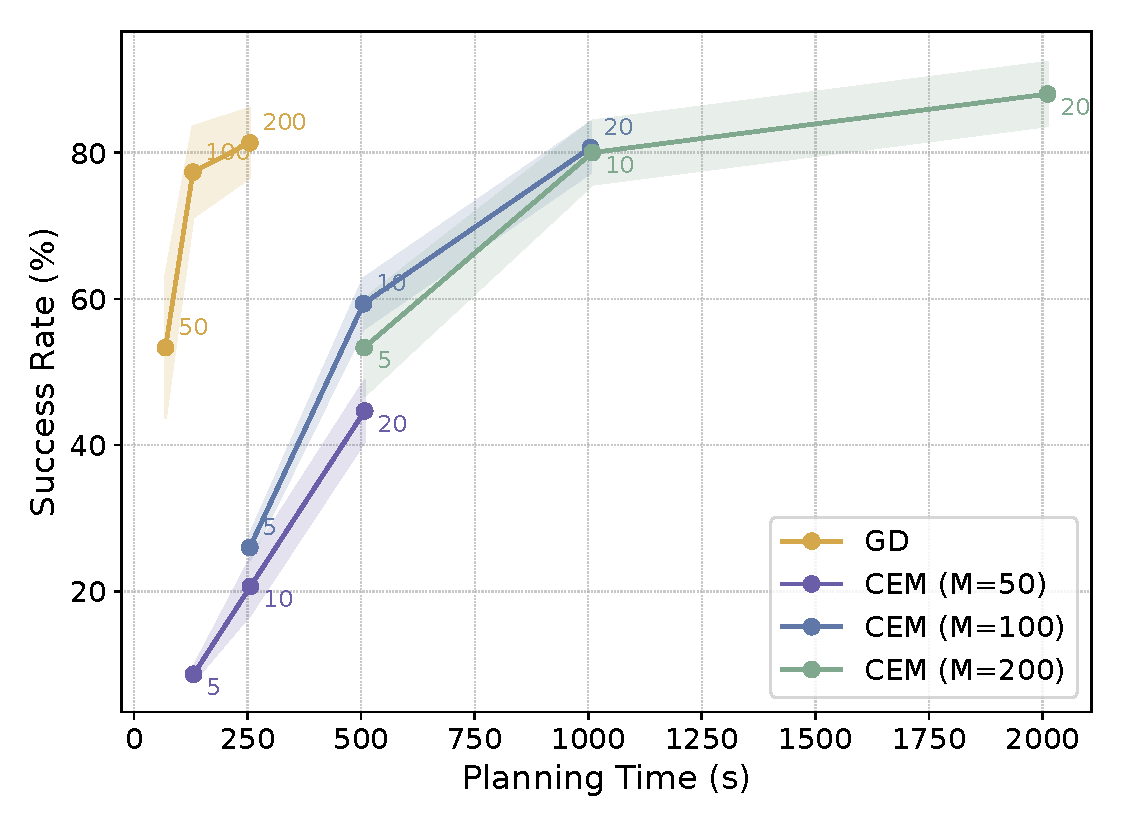
\includegraphics[width=\linewidth]{images/speed_vs_success.pdf}
\caption{Success rate versus wall-clock planning time for open-loop GD and CEM planning after straightening.}
\vspace{-0.2in}
\label{img:time}
\vspace{-0.1in}
\end{wrapfigure}

We compare the open-loop success rate using GD and CEM planners. For one single plan, GD optimizes the action sequence by backpropagating through the learned rollout model. With $N$ optimization steps, this requires $N$ forward rollouts and $N$ backward passes. In contrast, CEM iteratively samples $M$ candidate action sequences, rolls each candidate out with the learned predictor, refits the sampling distribution to the top-performing candidates, and repeats this procedure for $K$ iterations. Thus, CEM requires $MK$ forward rollouts, with $M$ typically large for competitive performance.

In our experiments, we find that CEM requires at least $200$ samples and $10$ iterations to achieve strong performance, making it roughly $10\times$ slower than GD in wall-clock planning time. We report wall-clock time for open-loop planning over 50 test trajectories on a single L40S GPU in~\Cref{img:time}.

As shown in~\Cref{tab:open_loop_gd_cem}, straightening consistently improves \textbf{both} GD and CEM across environments and model architectures. Consistent with prior work~\citep{dinowm}, CEM often obtains higher absolute success rates than GD, but at substantially higher computational cost. Importantly, straightening largely reduces the performance gap between GD and CEM, suggesting that the regularizer improves the latent optimization landscape and enables simple gradient-based planning to achieve a better success--latency trade-off.


\begin{table*}[h]
  \centering
  \caption{Goal-reaching Success Rate of 50 Test Trajectories (\%) in open-loop planning. We compare GD and CEM planners. Values are mean $\pm$ std over three data seeds. The best value is \textbf{bold}.}
  \label{tab:open_loop_gd_cem}
  \setlength{\tabcolsep}{5pt}
  \renewcommand{\arraystretch}{1.08}
  \resizebox{\linewidth}{!}{
  \begin{tabular}{lcc@{\hspace{8pt}}|@{\hspace{8pt}}cc@{\hspace{10pt}}cc@{\hspace{10pt}}cc@{\hspace{10pt}}cc}
    \toprule
    \multirow{2}{*}{Method} & \multicolumn{2}{c}{Config} &
    \multicolumn{2}{c}{Wall} &
    \multicolumn{2}{c}{PointMaze -- UMaze} &
    \multicolumn{2}{c}{PointMaze -- Medium} &
    \multicolumn{2}{c}{PushT} \\
    \cmidrule(lr){2-3}\cmidrule(lr){4-5}\cmidrule(lr){6-7}\cmidrule(lr){8-9}\cmidrule(lr){10-11}
     & dim & $\mathcal{L}_{curv}$ & GD & CEM & GD & CEM & GD & CEM & GD & CEM \\
    \midrule
    DINOv2 (patch) & $14 \times 14 \times 384$ & \xmark & 73.33 $\pm$ {\tiny 3.40} & 87.33 $\pm$ {\tiny 4.99} & 63.33 $\pm$ {\tiny 8.22} & 88.00 $\pm$ {\tiny 1.63} & 70.00 $\pm$ {\tiny 4.08} & 88.00 $\pm$ {\tiny 1.63} & 62.67 $\pm$ {\tiny 4.11} & 71.33 $\pm$ {\tiny 7.72} \\
    \rowcolor{Blue!5} DINOv2 (patch) + proj & $14 \times 14 \times 8$ & \xmark & 80.00 $\pm$ {\tiny 7.12} & 92.00 $\pm$ {\tiny 0.00} & 44.00 $\pm$ {\tiny 7.12} & 75.33 $\pm$ {\tiny 4.99} & 72.00 $\pm$ {\tiny 4.32} & \textbf{92.67} $\pm$ {\tiny 4.71} & 70.00 $\pm$ {\tiny 1.63} & 71.33 $\pm$ {\tiny 6.18} \\
    \rowcolor{Blue!5} DINOv2 (patch) + proj & $14 \times 14 \times 8$ & \cmark & \textbf{90.67} $\pm$ {\tiny 0.94} & \textbf{100.00} $\pm$ {\tiny 0.00} & \textbf{94.00} $\pm$ {\tiny 1.63} & \textbf{94.00} $\pm$ {\tiny 1.63} & \textbf{82.67} $\pm$ {\tiny 3.77} & 86.67 $\pm$ {\tiny 1.89} & \textbf{77.33} $\pm$ {\tiny 6.18} & \textbf{80.00} $\pm$ {\tiny 4.32} \\
    \rowcolor{Blue!5} ResNet & $14 \times 14 \times 8$ & \xmark & 1.33 $\pm$ {\tiny 1.89} & 1.33 $\pm$ {\tiny 0.94} & 14.67 $\pm$ {\tiny 4.99} & 20.67 $\pm$ {\tiny 0.94} & 18.67 $\pm$ {\tiny 4.11} & 24.00 $\pm$ {\tiny 4.32} & 71.33 $\pm$ {\tiny 7.36} & 56.00 $\pm$ {\tiny 0.00} \\
    \rowcolor{Blue!5} ResNet & $14 \times 14 \times 8$ & \cmark & 84.67 $\pm$ {\tiny 2.49} & 90.00 $\pm$ {\tiny 5.89} & 64.67 $\pm$ {\tiny 8.38} & 83.33 $\pm$ {\tiny 2.49} & 80.67 $\pm$ {\tiny 0.94} & 89.33 $\pm$ {\tiny 6.18} & 70.67 $\pm$ {\tiny 0.94} & 72.67 $\pm$ {\tiny 6.60} \\
    \bottomrule
  \end{tabular}
  }
\end{table*}




\newpage
\subsection{Effect of Feature Dimensions}
\label{app:ablations_dim}

In order to improve efficiency and efficacy, we ablate the output dimensions of the encoders. Here, we test on the ``frozen DINOv2 + spatial projector'' setup and preserve the spatial dimensions of the DINOv2 patch features $m_v=196$ but decreasing channels from 384 to $d_v \in \{2,8,32,128\}$. For all experiments, we use $lr=1e-6$ for the encoder. If with straightening, we apply straightening on the aggregation head as described in~\Cref{app:straightening} with a straightening strength $\lambda=0.1$. 

We report the open-loop planning success rate of 50 test samples over three data sampling seeds in~\Cref{img:ablation_dim}. Very small dimensions (e.g., \(d_v=2\)) result in poor performance, indicating insufficient capacity to preserve planning-relevant information. Increasing to a moderate dimension (\(d_v=\{8,32\}\)) yields the best results, while too large dimensions (\(d_v = 128\)) consistently reduce success rates. This suggests that overly high-dimensional latents can hinder gradient-based planning.

\begin{figure}[h]
\center
    \begin{subfigure}[t]{0.24\textwidth}
        \centering
        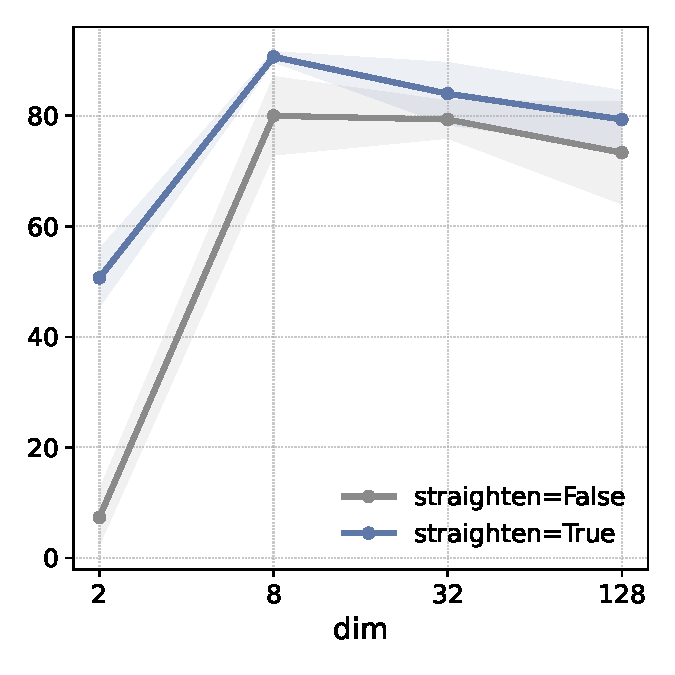
\includegraphics[width=\textwidth]{images/wall_both_projchannel_hw14_dim_curve.pdf}
        \caption{Wall}
        \label{fig:wall}
    \end{subfigure}
    \hfill
    \begin{subfigure}[t]{0.24\textwidth}
        \centering
        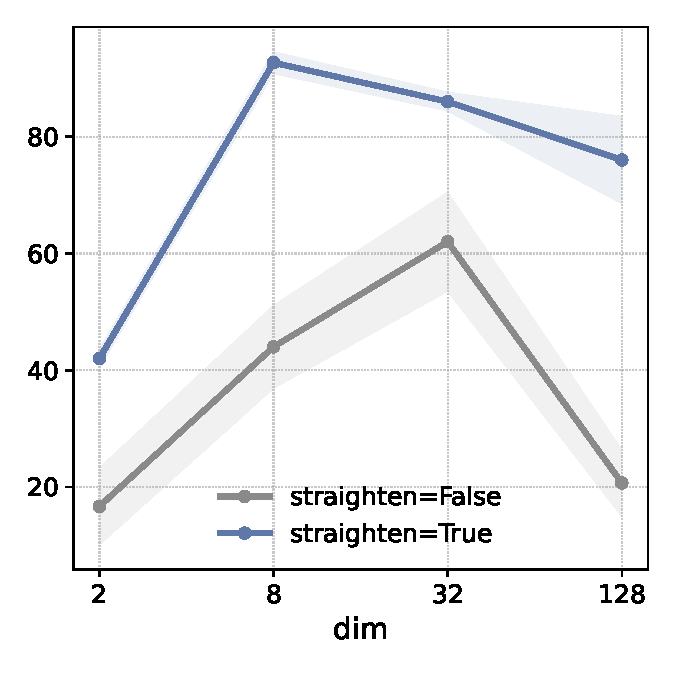
\includegraphics[width=\textwidth]{images/umaze_both_projchannel_hw14_dim_curve.pdf}
        \caption{PointMaze-UMaze}
        \label{fig:umaze}
    \end{subfigure}
    \hfill
    \begin{subfigure}[t]{0.24\textwidth}
        \centering
        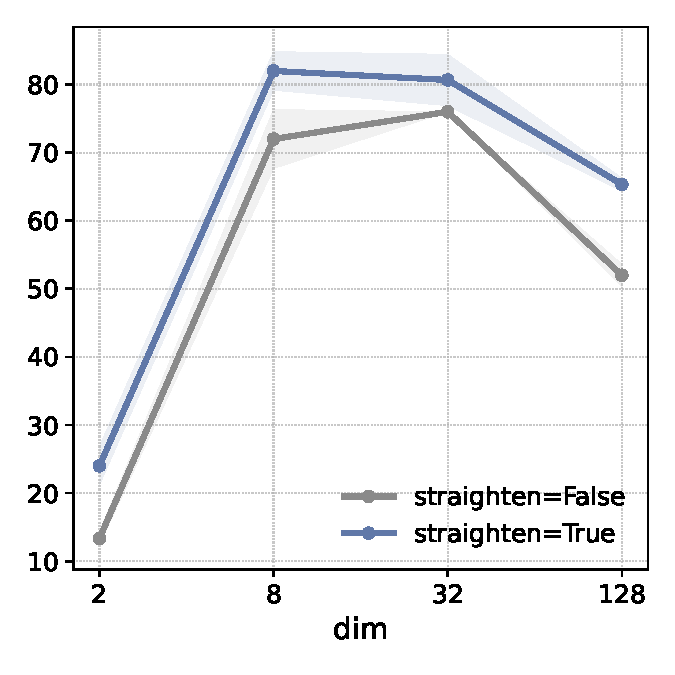
\includegraphics[width=\textwidth]{images/medium_both_projchannel_hw14_dim_curve.pdf}
        \caption{PointMaze-Medium}
        \label{fig:medium}
    \end{subfigure}
    \hfill
    \begin{subfigure}[t]{0.24\textwidth}
        \centering
        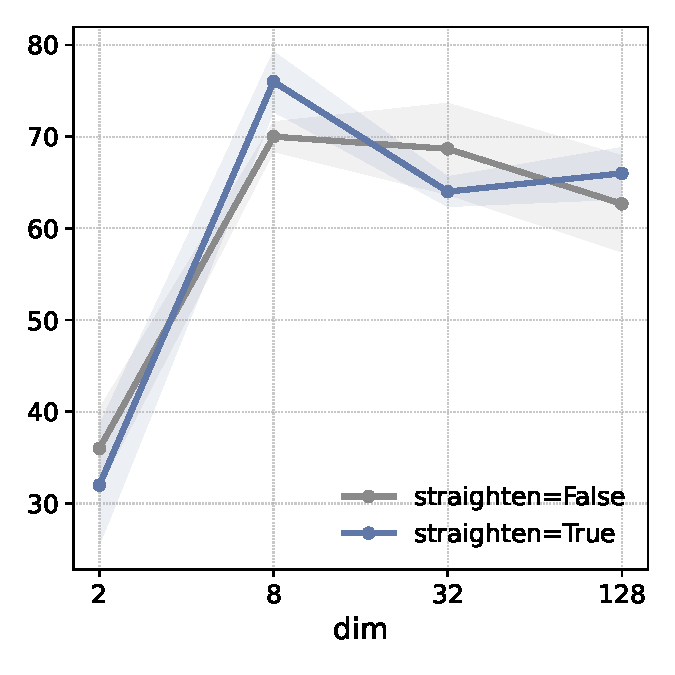
\includegraphics[width=\textwidth]{images/pusht_both_projchannel_hw14_dim_curve.pdf}
        \caption{PushT}
        \label{fig:mpc_pusht}
    \end{subfigure}
\caption{Comparison of Different Dimensions. The line plots show the success rate changes with increasing channels. Too small dimensions (e.g. $d_v=2$) are unable to encode sufficient planning-relevant information, while unnecessarily high dimensions (e.g. $d_v=128$) hinder the planning performance.
}
\label{img:ablation_dim}
\end{figure}

\subsection{Comparison to Smoothness and Temporal Contrastive Objectives}
\label{app:smooth_tc}

\begin{wrapfigure}{r}{0.3\textwidth}
\vspace{-0.3in}
\centering
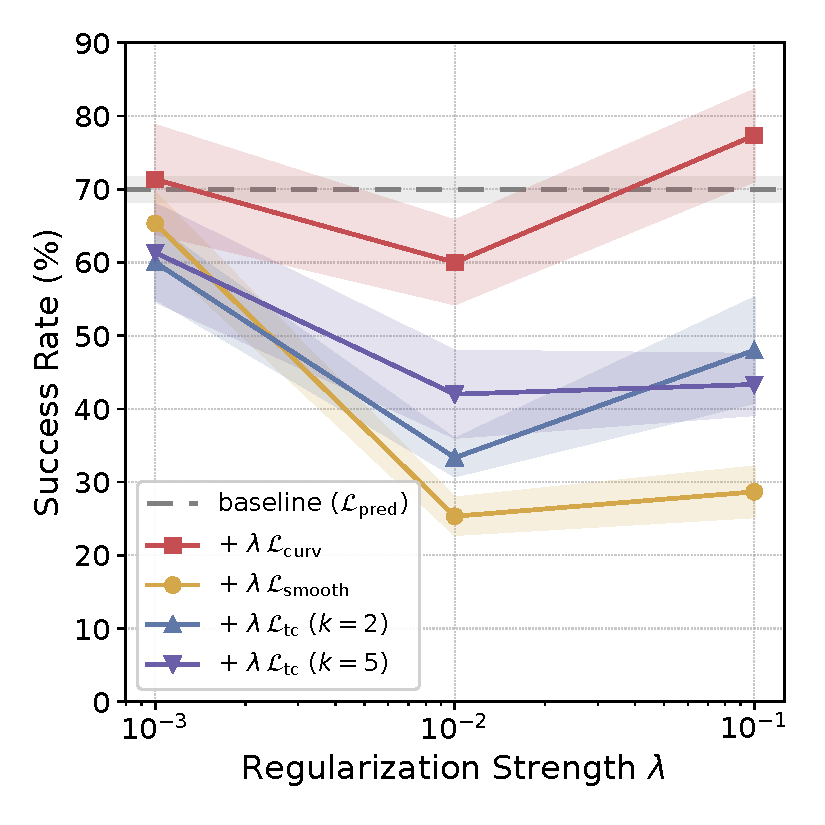
\includegraphics[width=\linewidth]{images/smooth_tc_ablation.pdf}
\caption{Comparison with Other Regularizations.}
\label{img:smmoth_tc}
\end{wrapfigure}

We compare with two common temporal regularization objectives:

\begin{itemize}
\item \textbf{Smoothness.} This objective penalizes large temporal jumps in visual embeddings:
\[
\mathcal{L}_{\mathrm{smooth}}=\mathbb{E}_t\left[\|z_{t+1}-z_t\|_2^2\right].
\]
However, an overly strong smoothness penalty can lead to degenerate solutions where embeddings of different states collapse to similar values.

\item \textbf{Time contrastiveness.} This objective treats frames within a temporal window of size $k$ as positives and other frames in the same trajectory as negatives, encouraging temporally nearby embeddings to be similar and temporally distant embeddings to be different:
\[
\mathcal{L}_{\mathrm{tc}}=\mathrm{InfoNCE}(z_{\mathrm{pos}},z_{\mathrm{neg}}).
\]
However, when training trajectories are suboptimal, temporal distance may not reflect geodesic distance: states that are geodesically close can be temporally far apart, and this objective may incorrectly separate them.
\end{itemize}

We test on the ``frozen DINOv2 + spatial projector'' setup and report open-loop GD planning success rate on PushT in~\Cref{img:smmoth_tc}, evaluated on 50 test samples over three data seeds. Overall, we do not observe improvements from adding smoothness or temporal contrastive objectives. Larger weights generally hurt performance, while smaller weights are less harmful but still do not match the gains from straightening. These objectives may still be useful in other settings, and our method is complementary to them: the curvature regularization loss can be combined with any other losses.

\clearpage

\subsection{Cosine Similarity Variants for Spatial Features}
\label{app:straightening}

\begin{wrapfigure}{r}{0.45\textwidth}
\vspace{-0.3in}
\centering
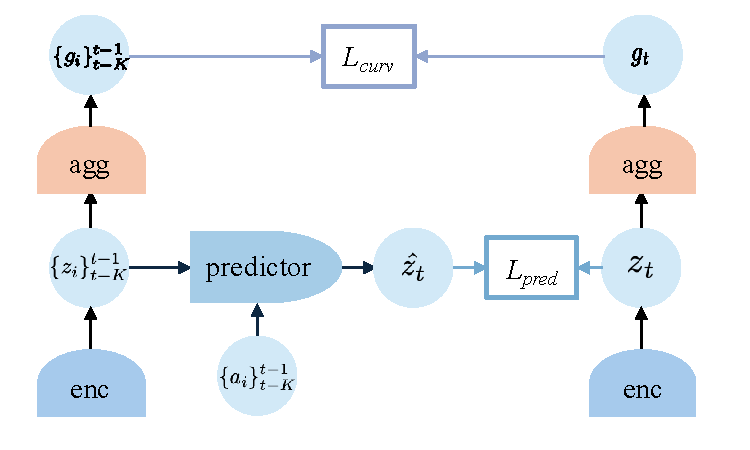
\includegraphics[width=\linewidth]{images/train_agg.pdf}
\caption{\colorbox{orange!20}{Aggregation Head} for Straightening during Training. The prediction loss is applied to spatial features, while the curvature loss is applied to the aggregated features.}
\label{img:agg}
\vspace{-0.5in}
\end{wrapfigure}

For spatial visual features \(z_t^v \in \mathbb{R}^{m_v \times d_v}\) (\(m_v>1\)), we compute straightness from approximate latent velocities
\(
v_t := z_{t+1}^v - z_t^v \in \mathbb{R}^{m_v \times d_v}.
\)
Let \(v_{t,i}\in\mathbb{R}^{d_v}\) denote the \(i\)-th patch vector and \(\cos(u,w)=\frac{u^\top w}{\|u\|_2\|w\|_2}\). We ablate four choices of \(\mathcal{C}_t\):


\begin{itemize}

\item \textbf{[patch]} We treat each patch independently, then average:
\[
\mathcal{C}_t=\frac{1}{m_v}\sum_{i=1}^{m_v}\cos\!\left(v_{t,i},\,v_{t+1,i}\right).
\]

\item \textbf{[mean]} We average patches to one vector, then cosine:
\[
\bar v_t=\frac{1}{m_v}\sum_{i=1}^{m_v} v_{t,i},
\qquad
\mathcal{C}_t=\cos(\bar v_t,\bar v_{t+1}).
\]
\end{itemize}

\begin{itemize}
\item \textbf{[flatten]} We flatten the spatial features and compute a single cosine over all dimensions:
\[
\mathcal{C}_t=\cos\!\left(\mathrm{vec}(v_t),\,\mathrm{vec}(v_{t+1})\right),
\]
where \(\mathrm{vec}(\cdot):\mathbb{R}^{m_v\times d_v}\to\mathbb{R}^{m_v d_v}\).

\item \textbf{[agg]} We learn an aggregation head to aggregate features to a single global feature before cosine (\Cref{img:agg}):
\[
\mathcal{C}_t=\cos\!\left(h_\phi(v_t),\,h_\phi(v_{t+1})\right),
\]
with an aggregation head \(h_\phi:\mathbb{R}^{m_v\times d_v}\to\mathbb{R}^{d_h}\). Concretely, we use an MLP with an output dimension of 128 as $h_\phi$ in all experiments.
\end{itemize}

We test these variants on the ``frozen DINOv2 + spatial projector'' setup and report the open-loop planning success rate of 50 test samples over three data sampling seeds in~\Cref{img:ablation_str}. The projector projects pretrained DINOv2 patch features $e_t \in \mathbb{R}^{196\times384}$ to $z_t \in \mathbb{R}^{196\times8}$. For the straightening strength coefficient, we use $\lambda=0.1$ for agg and $\lambda=0.01$ for the rest, as these values yield the best performance. We find that using a learnable aggregation head performs best. This is not surprising as straightening should act on the \emph{global} trajectory representations, whereas spatial tokens mainly capture local, patch-level variations that are only loosely aligned across time due to object motion and occlusion.

\begin{figure}[h]
\center
    \begin{subfigure}[t]{0.24\textwidth}
        \centering
        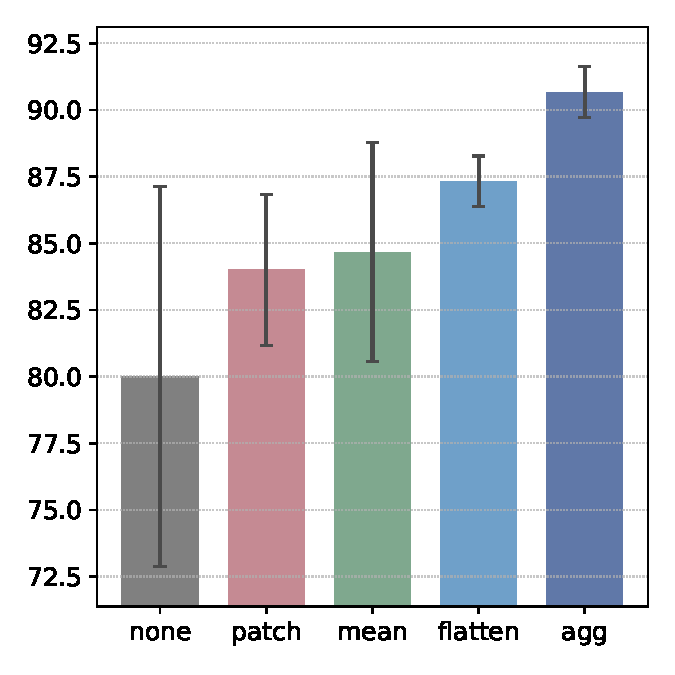
\includegraphics[width=\textwidth]{images/wall_dim8_hw14_straightening_bar.pdf}
        \caption{Wall}
        \label{fig:wall}
    \end{subfigure}
    \hfill
    \begin{subfigure}[t]{0.24\textwidth}
        \centering
        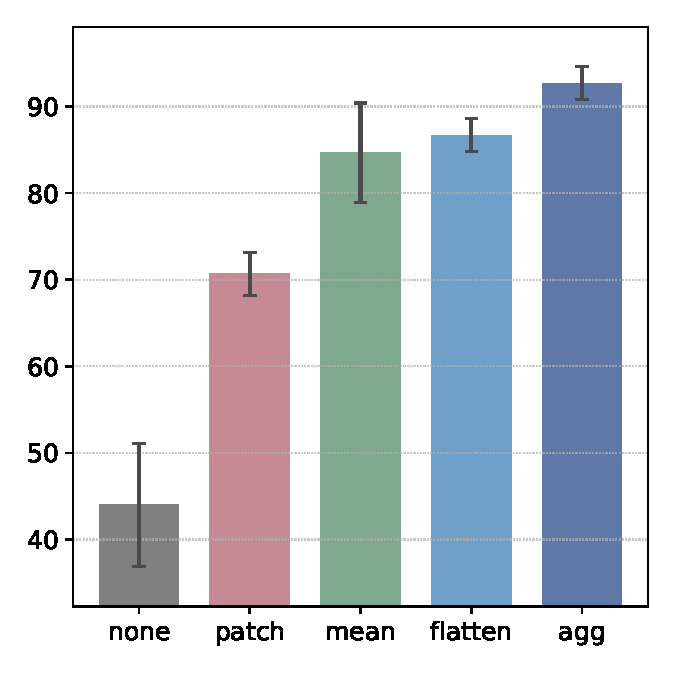
\includegraphics[width=\textwidth]{images/umaze_dim8_hw14_straightening_bar.pdf}
        \caption{PointMaze-UMaze}
        \label{fig:umaze}
    \end{subfigure}
    \hfill
    \begin{subfigure}[t]{0.24\textwidth}
        \centering
        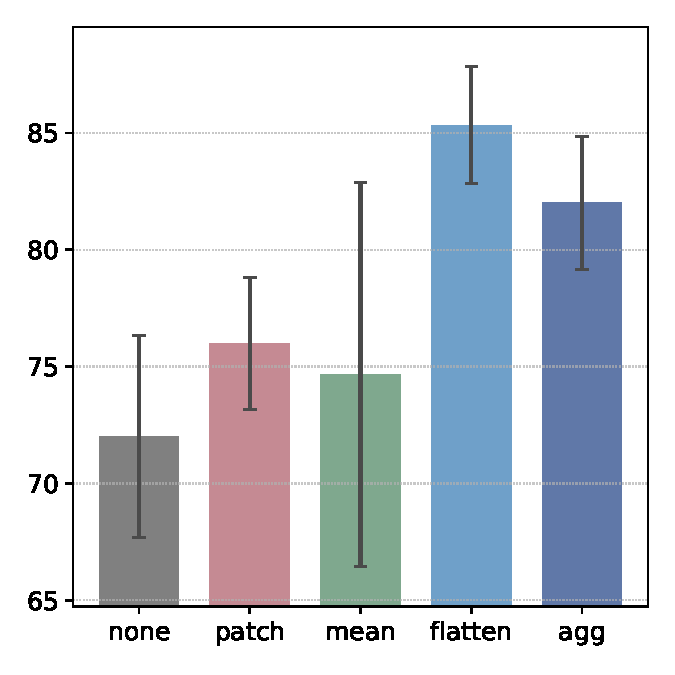
\includegraphics[width=\textwidth]{images/medium_dim8_hw14_straightening_bar.pdf}
        \caption{PointMaze-Medium}
        \label{fig:medium}
    \end{subfigure}
    \hfill
    \begin{subfigure}[t]{0.24\textwidth}
        \centering
        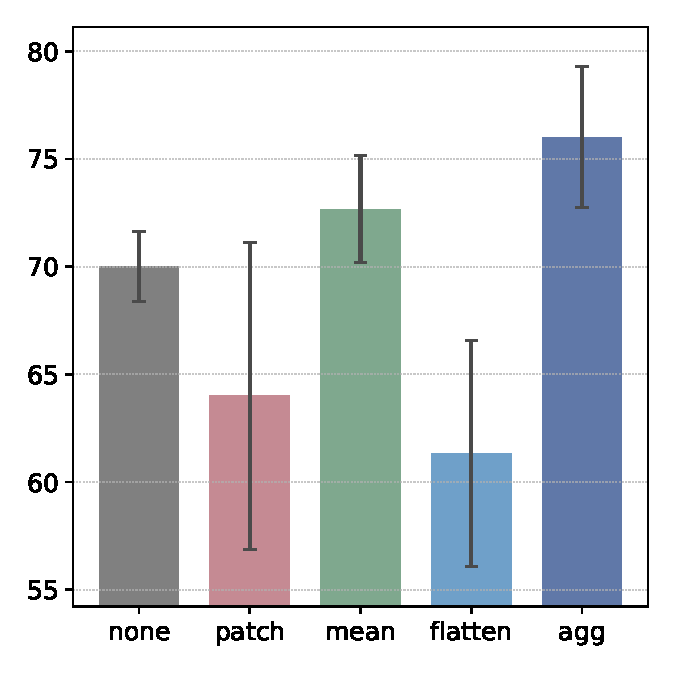
\includegraphics[width=\textwidth]{images/pusht_dim8_hw14_straightening_bar.pdf}
        \caption{PushT}
        \label{fig:mpc_pusht}
    \end{subfigure}
\caption{Comparison of Different Straightening Strategies. The bar charts show the planning success rates. While all cosine similarity variants lead to better performance than no straightening, adding a learnable aggregation head gives the best performance.
}
\label{img:ablation_str}
\end{figure}

\clearpage




\section{Theoretical Analysis}

\subsection{Setup and notation}
We optimize an action sequence $\mathbf a=(a_0,\dots,a_{K-1})\in\mathbb{R}^{K\times d_a}$ over horizon $K$
to minimize the terminal MSE
\begin{equation}\label{eq:app_obj}
\mathcal L(\mathbf a)=\|z_K-z_g\|_2^2,\qquad z_K=\Phi(\mathbf a),
\end{equation}
where $\Phi$ denotes unrolling the latent dynamics from a fixed initial state $z_0$.

\begin{assumption}[Linear latent dynamics]\label{as:app_linear}
We assume linear latent dynamics
\begin{equation}\label{eq:app_linear}
z_{t+1}=Az_t+Ba_t,\qquad A\in\mathbb{R}^{d\times d},\; B\in\mathbb{R}^{d\times d_a}.
\end{equation}
\end{assumption}

\begin{definition}[Effective condition number]\label{def:app_keff}
For a PSD matrix $H\succeq 0$ with a nontrivial nullspace, define
\[
\kappa_{\mathrm{eff}}(H):=\frac{\sigma_{\max}(H)}{\sigma_{\min}^+(H)},
\]
where $\sigma_{\min}^+(H)$ is the smallest nonzero singular value.
\end{definition}

\begin{definition}[$\varepsilon$-straight transition]\label{def:app_eps}
In the linear model~\eqref{eq:app_linear}, define
\[
\varepsilon:=\|A-I\|_2.
\]
\end{definition}

\subsection{Conditioning of the planning Hessian}
\label{app:theory_hessian}

Unrolling~\eqref{eq:app_linear} gives the affine terminal map
\begin{equation}\label{eq:app_unroll}
z_K
=
A^{K} z_0 + \sum_{t=0}^{K-1} A^{K-1-t} B a_t.
\end{equation}
Define the rollout Jacobian
\begin{equation}\label{eq:app_Jphi}
J_\Phi
:=
\frac{\partial z_K}{\partial \mathbf a}
=
\bigl[\,A^{K-1}B,\quad A^{K-2}B,\quad \cdots,\quad B\,\bigr]
\in\mathbb{R}^{d\times (K d_a)}.
\end{equation}
The associated finite-horizon discrete controllability Gramian is
\begin{equation}\label{eq:app_gram}
\mathcal W_K
:=
J_\Phi J_\Phi^\top
=
\sum_{k=0}^{K-1} A^k B B^\top (A^\top)^k\in\mathbb{R}^{d\times d},
\end{equation}
a standard term in linear systems~\citep{kailath1980linear,sontag1998mathematical,chen1999linear}.

\begin{lemma}[Hessian form and Gramian equivalence]\label{lem:app_hess_gram}
Under~\eqref{eq:app_obj}--\eqref{eq:app_linear}, the planning Hessian satisfies
\begin{equation}\label{eq:app_hess}
H:=\nabla^2_{\mathbf a}\mathcal L(\mathbf a)=2J_\Phi^\top J_\Phi\succeq 0.
\end{equation}
Moreover, the nonzero singular values of $J_\Phi^\top J_\Phi$ equal those of $J_\Phi J_\Phi^\top$,
hence
\begin{equation}\label{eq:app_keff_equal}
\kappa_{\mathrm{eff}}(H)=\kappa(\mathcal W_K).
\end{equation}
\end{lemma}

\begin{proof}
$H$ is positive semi-definite by definition. Since $z_K$ is affine in $\mathbf a$ by~\eqref{eq:app_unroll},
$\mathcal L(\mathbf a)=\|z_K-z_g\|_2^2$ is a convex quadratic, and direct differentiation yields
$H=2J_\Phi^\top J_\Phi\succeq 0$.
For any matrix $M$, the nonzero eigenvalues of $M^\top M$ and $MM^\top$ coincide.
Applying this with $M=J_\Phi$ gives that the nonzero eigenvalues of $H/2$ equal those of $\mathcal W_K$,
which implies~\eqref{eq:app_keff_equal}.
\end{proof}

\begin{theorem}[Conditioning bound]\label{thm:app_cond}
Assume~\eqref{eq:app_linear}. Consider first the square-action case $d_a=d$ with $B$ invertible.
Then
\begin{equation}\label{eq:app_kappaA}
\kappa_{\mathrm{eff}}(H)=\kappa(\mathcal W_K)
\;\le\;
\kappa(B)^2\,
\frac{\sum_{k=0}^{K-1}\sigma_{\max}(A)^{2k}}{\sum_{k=0}^{K-1}\sigma_{\min}(A)^{2k}}
\;\le\;
\kappa(B)^2\,\kappa(A)^{2(K-1)},
\end{equation}
where $\kappa(A):=\sigma_{\max}(A)/\sigma_{\min}(A)$.
If additionally $\varepsilon=\|A-I\|_2<1$, then
\begin{equation}\label{eq:app_eps}
\kappa_{\mathrm{eff}}(H)
\;\le\;
\kappa(B)^2\left(\frac{1+\varepsilon}{1-\varepsilon}\right)^{2(K-1)}
\;\le\;
\kappa(B)^2 e^{6\varepsilon K}
\quad(\varepsilon\le\tfrac12).
\end{equation}
\end{theorem}

\begin{proof}
By Lemma~\ref{lem:app_hess_gram}, it suffices to bound $\kappa(\mathcal W_K)$.

\paragraph{Upper bound.}
For any unit vector $x\in\mathbb{R}^d$,
\[
x^\top \mathcal W_K x = \sum_{k=0}^{K-1}\|B^\top (A^\top)^k x\|_2^2
\le
\sum_{k=0}^{K-1}\|B\|_2^2\|A^k\|_2^2\|x\|_2^2
\le
\sigma_{\max}(B)^2\sum_{k=0}^{K-1}\sigma_{\max}(A)^{2k}.
\]
Taking the maximum over $\|x\|_2=1$ yields
\[
\lambda_{\max}(\mathcal W_K)\le \sigma_{\max}(B)^2\sum_{k=0}^{K-1}\sigma_{\max}(A)^{2k}.
\]

\paragraph{Lower bound.}
Since $B$ is invertible, $\|B^\top u\|_2\ge \sigma_{\min}(B)\|u\|_2$ for all $u$.
Also $\sigma_{\min}(A^k)\ge \sigma_{\min}(A)^k$. Thus for any unit $x$,
\[
\|B^\top(A^\top)^k x\|_2
\ge
\sigma_{\min}(B)\,\|(A^\top)^k x\|_2
\ge
\sigma_{\min}(B)\,\sigma_{\min}(A^k)\,\|x\|_2
\ge
\sigma_{\min}(B)\,\sigma_{\min}(A)^k,
\]
hence
\[
x^\top \mathcal W_K x
\ge
\sigma_{\min}(B)^2\sum_{k=0}^{K-1}\sigma_{\min}(A)^{2k}.
\]
Taking the minimum over $\|x\|_2=1$ yields
\[
\lambda_{\min}(\mathcal W_K)\ge \sigma_{\min}(B)^2\sum_{k=0}^{K-1}\sigma_{\min}(A)^{2k}.
\]

\paragraph{Combine.}
Dividing the two bounds gives the first inequality in~\eqref{eq:app_kappaA}.
For the second, use positivity of terms:
\[
\frac{\sum_{k=0}^{K-1}\sigma_{\max}(A)^{2k}}{\sum_{k=0}^{K-1}\sigma_{\min}(A)^{2k}}
\le
\max_{0\le k\le K-1}\frac{\sigma_{\max}(A)^{2k}}{\sigma_{\min}(A)^{2k}}
=
\kappa(A)^{2(K-1)}.
\]

\paragraph{$\varepsilon$-specialization.}
If $\varepsilon=\|A-I\|_2<1$, then by Weyl's perturbation theorem,
$\sigma_{\max}(A)\le 1+\varepsilon$ and $\sigma_{\min}(A)\ge 1-\varepsilon$,
which implies the first inequality in~\eqref{eq:app_eps}.
For $\varepsilon\le \tfrac12$, the standard bound
$\ln\!\big(\frac{1+\varepsilon}{1-\varepsilon}\big)\le 3\varepsilon$
gives the exponential form.
\end{proof}

\begin{remark}[Low-dimensional actions $d_a<d$]\label{rem:app_lowdim}
If $d_a<d$, then $B$ is not invertible and $\mathcal W_K$ may be singular.
All statements hold on the controllable subspace
$\mathcal S_K=\mathrm{range}(\mathcal W_K)$ by replacing $\lambda_{\min}(\mathcal W_K)$ with
$\lambda_{\min}^+(\mathcal W_K)$ and interpreting $\kappa(\mathcal W_K)$ as an effective condition number.
In this case, additional controllability assumptions are needed to lower bound $\sigma_{\min}^+(\mathcal W_K)$.
\end{remark}

\subsection{Cosine similarity as a proxy}
\label{app:theory_cos}

\begin{assumption}[Constant velocity and smooth actions]\label{as:app_cos_const}
Define latent velocities $v_t:=z_{t+1}-z_t$. Assume there exists a constant $c>0$ such that
\[
\|v_t\|_2=c\qquad \text{for all } t=0,\dots,K-1.
\]
Assume action smoothness $\Delta_a:=\max_{t}\|a_{t+1}-a_t\|_2<\infty$.
\end{assumption}

\begin{definition}[Cosine similarity]\label{def:app_cos}
For $t=0,\dots,K-2$, define
\[
\mathcal C_t:=\cos(v_t,v_{t+1})
=\frac{v_t^\top v_{t+1}}{\|v_t\|_2\|v_{t+1}\|_2},
\qquad
\bar{\mathcal C}:=\frac{1}{K-1}\sum_{t=0}^{K-2}\mathcal C_t.
\]
\end{definition}

\begin{proposition}[Cosine proxy $\Rightarrow$ small $(A-I)$ along visited directions]\label{prop:app_cos}
Under linear dynamics~\eqref{eq:app_linear}, let $\hat v_t:=v_t/\|v_t\|_2$.
Under Assumption~\ref{as:app_cos_const}, for each $t=0,\dots,K-2$,
\begin{equation}\label{eq:app_dir_point_const}
\|(A-I)\hat v_t\|_2
\;\le\;
\sqrt{2(1-\mathcal C_t)}
\;+\;
\frac{\sigma_{\max}(B)\Delta_a}{c}.
\end{equation}
If $\bar{\mathcal C}\ge 1-\eta$, then
\begin{equation}\label{eq:app_dir_avg_const}
\frac{1}{K-1}\sum_{t=0}^{K-2}\|(A-I)\hat v_t\|_2
\;\le\;
\sqrt{2\eta}
\;+\;
\frac{\sigma_{\max}(B)\Delta_a}{c}.
\end{equation}
\end{proposition}

\begin{proof}
Under~\eqref{eq:app_linear},
\[
v_{t+1}-v_t
=
(z_{t+2}-z_{t+1})-(z_{t+1}-z_t)
=
(A-I)(z_{t+1}-z_t)+B(a_{t+1}-a_t)
=
(A-I)v_t+B(a_{t+1}-a_t).
\]
Thus, by the triangle inequality,
\[
\|(A-I)\hat v_t\|_2
=
\frac{\|(A-I)v_t\|_2}{\|v_t\|_2}
\le
\frac{\|v_{t+1}-v_t\|_2}{\|v_t\|_2}
+
\frac{\|B(a_{t+1}-a_t)\|_2}{\|v_t\|_2}
\le
\frac{\|v_{t+1}-v_t\|_2}{c}
+
\frac{\sigma_{\max}(B)\Delta_a}{c}.
\]
Since $\|v_t\|_2=\|v_{t+1}\|_2=c$,
\[
\|v_{t+1}-v_t\|_2^2
=
\|v_{t+1}\|_2^2+\|v_t\|_2^2-2v_{t+1}^\top v_t
=
2c^2(1-\mathcal C_t),
\]
hence $\|v_{t+1}-v_t\|_2/c=\sqrt{2(1-\mathcal C_t)}$, proving~\eqref{eq:app_dir_point_const}.
Averaging and applying Jensen's inequality to the concave map $x\mapsto\sqrt{x}$ gives
\[
\frac{1}{K-1}\sum_{t=0}^{K-2}\sqrt{1-\mathcal C_t}
\le
\sqrt{1-\bar{\mathcal C}}
\le
\sqrt{\eta},
\]
which implies~\eqref{eq:app_dir_avg_const}.
\end{proof}

\begin{remark}[Directional vs.\ spectral control]\label{rem:app_dir_vs_spec}
Proposition~\ref{prop:app_cos} bounds $(A-I)$ only along visited directions $\{\hat v_t\}$. Upgrading this to a uniform spectral bound $\varepsilon=\|A-I\|_2$ requires an additional coverage condition so that visited directions span the latent space. This is not an unreasonable assumption since training trajectories are typically collected to be diverse. Under such regimes, maximizing cosine similarity provides a meaningful proxy for making $A$ close to $I$ in spectral norm.
\end{remark}

\section{Related Work (Cont.) }
\label{sec:related_cont}

Here, we discuss the connections and differences between temporal straightening and local linearization, Koopman methods, and the broader literature on learning plannable representations. Temporal straightening targets the curvature of latent trajectories, a geometric property distinct from linear dynamics, whether local or global.

Local model-based control approximates nonlinear dynamics around a nominal trajectory using first- or second-order models, as in DDP and iLQR \citep{mayne1966ddp,li2004ilqr}. Because these methods presuppose a low-dimensional state space, they have motivated representation-learning methods that map high-dimensional observations into latent spaces where local dynamics models become applicable. For example, E2C and RCE explicitly impose locally linear latent dynamics \citep{watter2015embedcontrollocallylinear,banijamali2018robust}, while later methods broaden this direction by learning representations or objectives that support locally linear control \citep{zhang2019solar,Levine2020pcc,shu2020pc3}. Temporal straightening differs in both goal and mechanism. We do not aim to learn locally linear dynamics, nor do we design representations for locally linear control. Instead, we jointly learn the encoder and predictor while directly regularizing the geometry of latent trajectories.

Koopman methods seek observables whose evolution is linear under a global operator \citep{koopman1931hamiltonian}. Recent deep models learn such observables or eigenfunctions directly from data \citep{lusch2018koopman,yeung2019koopman,takeishi2017learning,cheng2026information}. Temporal straightening targets a different property of the learned representation. Koopman methods constrains the form of the dynamics model but do not require latent trajectories to be straight as linear systems can still produce curved or oscillatory paths. In contrast, temporal straightening allows nonlinear latent dynamics through a learned predictor, but more directly regularizes trajectory geometry by penalizing curvature along observed transitions.

More broadly, our work is related to learning plannable representations, especially methods that make planning easier by aligning latent geometry or value structure with feasible transitions. This includes approaches where planning or inference can be carried out through interpolation in latent space \citep{eysenbach2024inference,kurutach2018causalinfogan,wang2019visualplanning}, as well as methods that build planning-oriented geometry from shortest-path, reachability, or asymmetric goal-reaching structure \citep{yang2020plan2vec,wang2023quasimetric}. These works share the premise that representation geometry or value structure matters for planning, but with different focuses. Our contribution is to use straightening itself as a simple geometry regularization during training.




\clearpage
\section{Visualizations}

\subsection{Distance Heatmaps}
\label{app:heatmap}

We plot heatmaps of the Euclidean distances in the embedding space. The yellow star represents the target, and we compute the Euclidean distance between its embedding and those of all other states in the maze. Blue indicates small values, and red indicates large values. With straightening, the latent distance accurately reflects the minimum number of steps required to reach the target. We find that spatial and global/aggregated features capture complementary distance information: spatial features preserve local geometry and yield fine-grained, locally discriminative distances, while global/aggregated features provide an informative longer-range signal.

We compare the distance heatmaps with ground-truth heatmaps constructed by dividing the mazes into discrete grids and applying the A-star algorithm. 4-neighbor connectivity means each grid cell connects only to up/down/left/right cells. 8-neighbor connectivity adds the four diagonals (up-left, up-right, down-left, down-right), so paths can cut corners diagonally and distances are usually shorter.

\begin{figure}[h]
\center
    \begin{subfigure}[t]{0.46\textwidth}
        \centering
        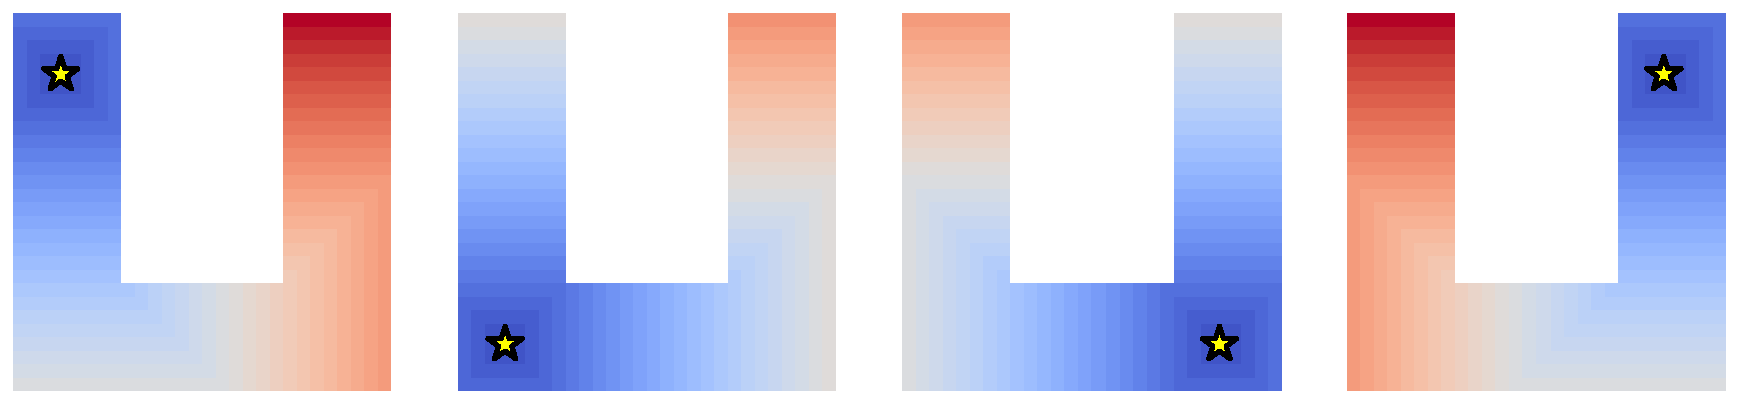
\includegraphics[width=\textwidth]{images/heatmap/umaze_geo8_gt.pdf}
        \caption{Ground-Truth using A-star (4 neighbors)}
    \end{subfigure}
    \hfill
    \begin{subfigure}[t]{0.46\textwidth}
        \centering
        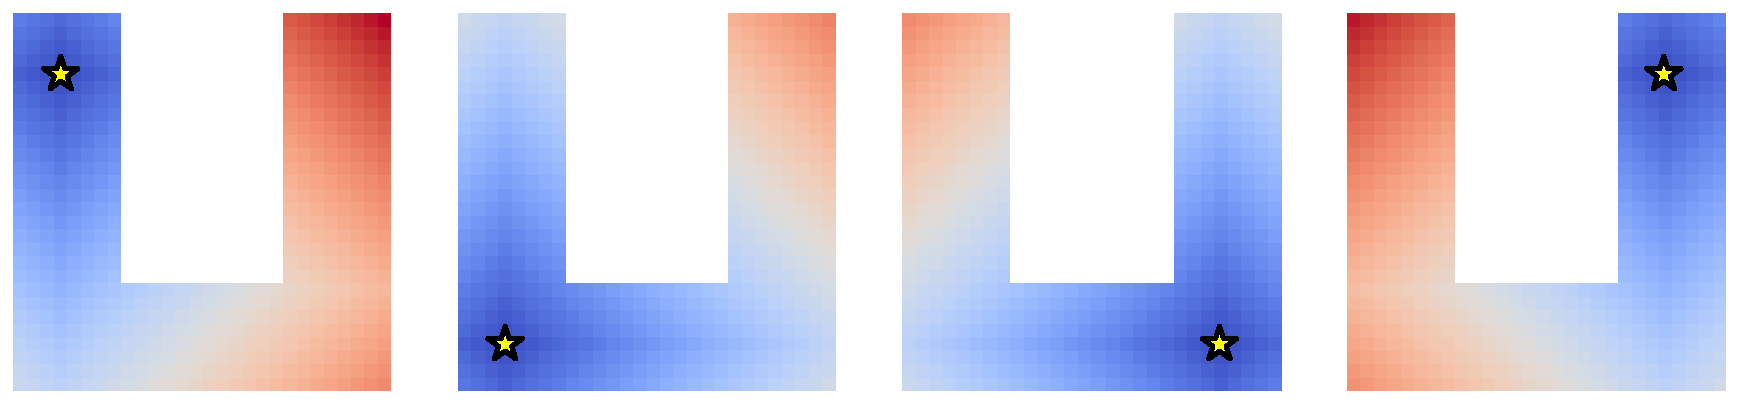
\includegraphics[width=\textwidth]{images/heatmap/umaze_geo4_gt.pdf}
        \caption{Ground-Truth using A-star (8 neighbors)}
    \end{subfigure}
    \begin{subfigure}[t]{0.46\textwidth}
        \centering
        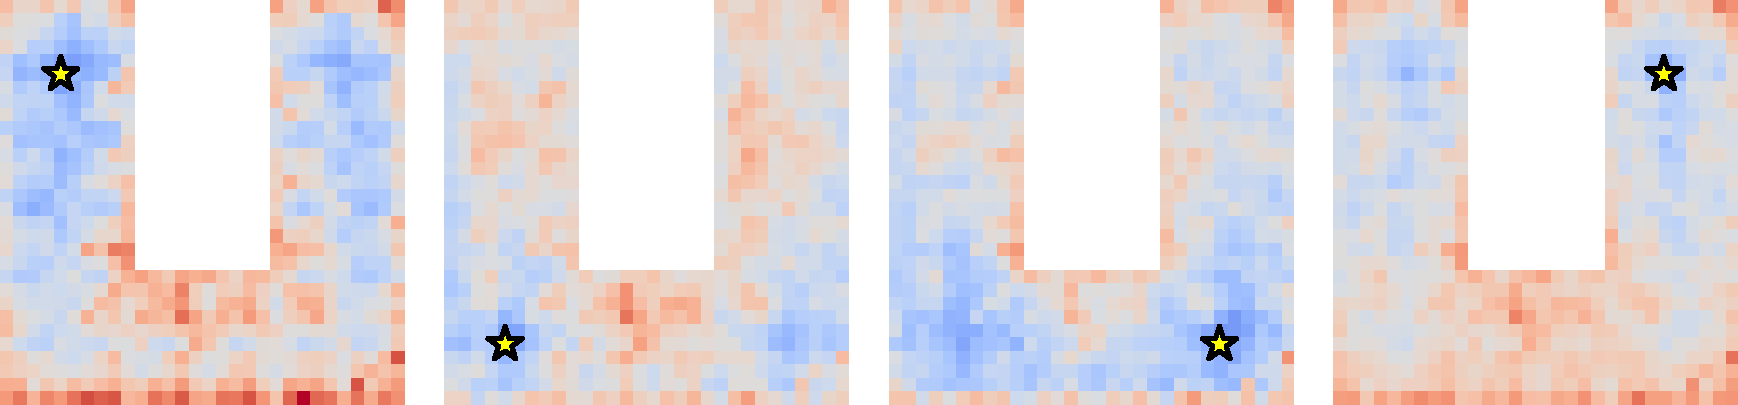
\includegraphics[width=\textwidth]{images/heatmap/umaze_dino_cls.pdf}
        \caption{DINOv2 CLS embedding}
    \end{subfigure}
    \hfill
    \begin{subfigure}[t]{0.46\textwidth}
        \centering
        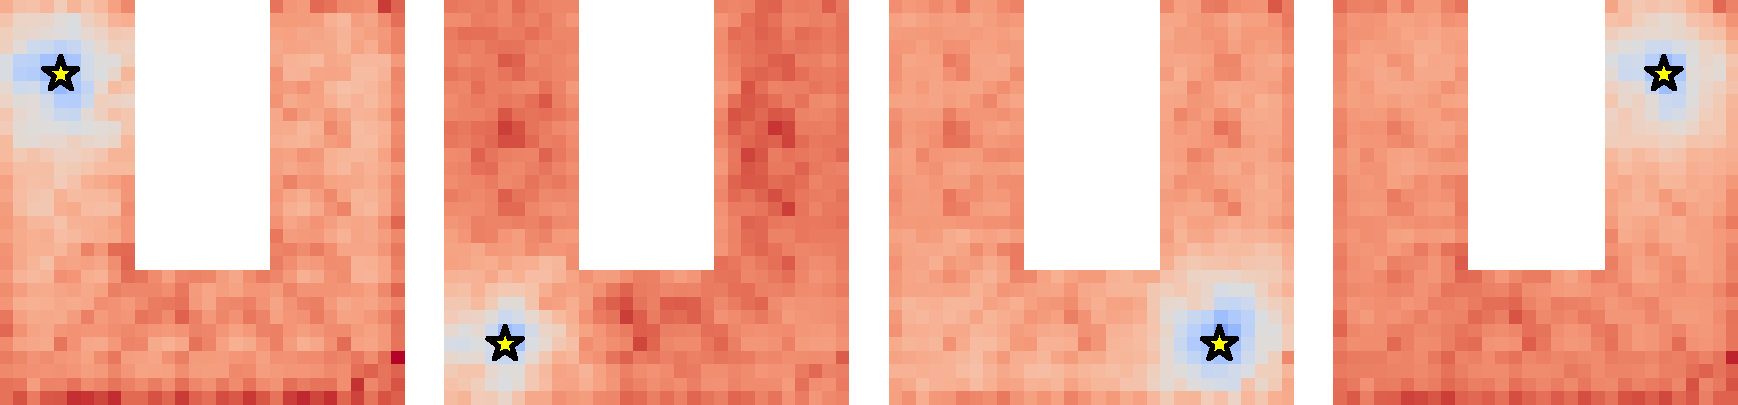
\includegraphics[width=\textwidth]{images/heatmap/umaze_dino_patch.pdf}
        \caption{DINOv2 patch embedding}
    \end{subfigure}
    \begin{subfigure}[t]{0.46\textwidth}
        \centering
        
\includegraphics[width=\textwidth]{images/heatmap/proj/umaze_False_projchannel_dim8_hw14/patch.pdf}
        \caption{DINOv2 + spatial proj [straightening=False]}
    \end{subfigure}
    \hfill
    \begin{subfigure}[t]{0.46\textwidth}
        \centering
        
\includegraphics[width=\textwidth]{images/heatmap/resnet/umaze_False_resnetplus_dim8_hw14_sgTrue_lr1e-5/patch.pdf}
        \caption{ResNet - spatial [straightening=False]}
    \end{subfigure}
        \begin{subfigure}[t]{0.46\textwidth}
        \centering
        
\includegraphics[width=\textwidth]{images/heatmap/resnet/umaze_False_resnet_dim384_hw1_sgTrue/global.pdf}
        \caption{ResNet - global [straightening=False]}
    \end{subfigure}
    \hfill
    \begin{subfigure}[t]{0.46\textwidth}
        \centering
        
\includegraphics[width=\textwidth]{images/heatmap/resnet/umaze_cos1e-1_resnet_dim384_hw1_sgTrue/global.pdf}
        \caption{ResNet - global [straightening=True]}
    \end{subfigure}
    \begin{subfigure}[t]{0.46\textwidth}
        \centering
        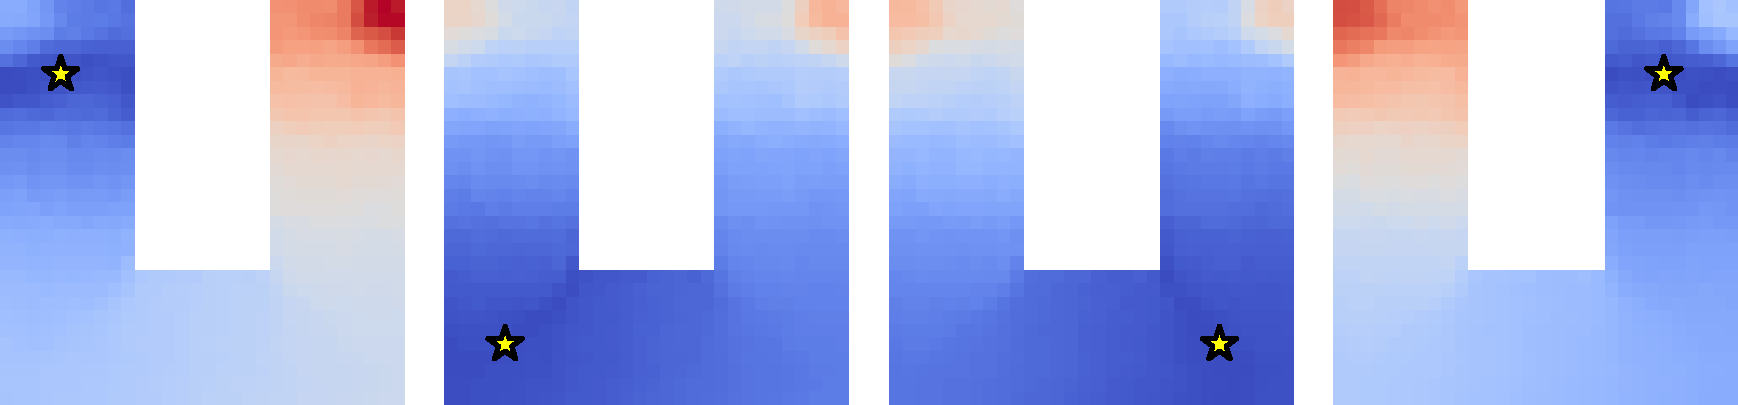
\includegraphics[width=\textwidth]{images/heatmap/proj/umaze_aggmlpcos1e-1_projchannel_dim8_hw14/20_agg.pdf}
        \caption{DINOv2 + spatial proj (agg head) [straightening=True]}
    \end{subfigure}
    \hfill
    \begin{subfigure}[t]{0.46\textwidth}
        \centering
        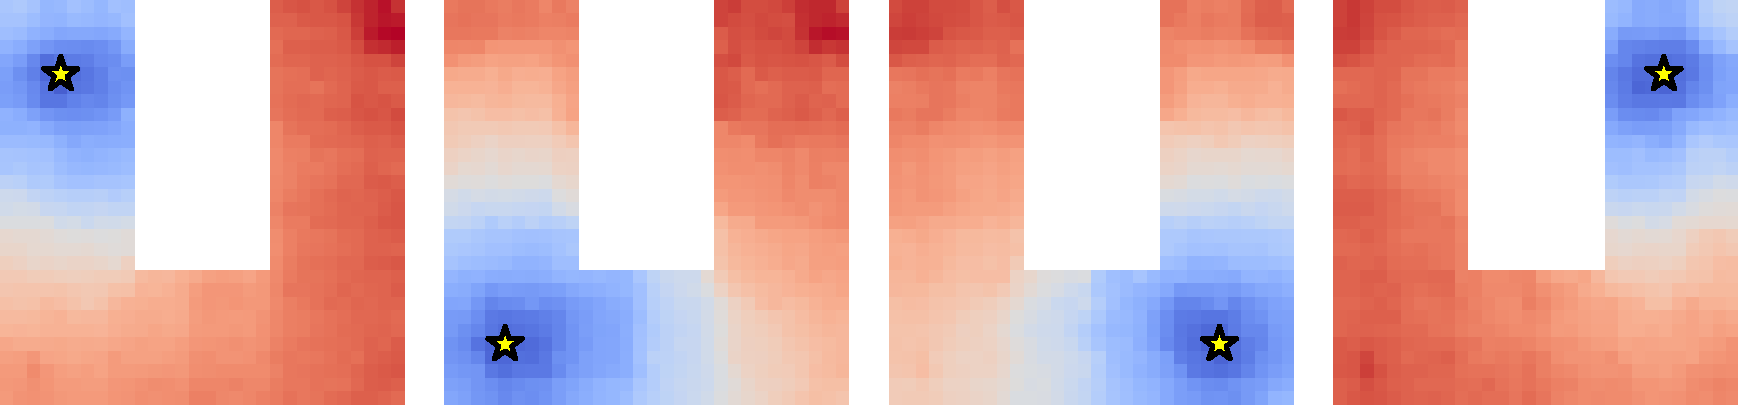
\includegraphics[width=\textwidth]{images/heatmap/proj/umaze_aggmlpcos1e-1_projchannel_dim8_hw14/20_patch.pdf}
        \caption{DINOv2 + spatial proj (spatial) [straightening=True]}
    \end{subfigure}
        \begin{subfigure}[t]{0.46\textwidth}
        \centering
        
\includegraphics[width=\textwidth]{images/heatmap/resnet/umaze_aggmlpcos1e-1_resnetplus_dim8_hw14/20_agg.pdf}
        \caption{ResNet - spatial (agg head) [straightening=True]}
    \end{subfigure}
    \hfill
    \begin{subfigure}[t]{0.46\textwidth}
        \centering
        
\includegraphics[width=\textwidth]{images/heatmap/resnet/umaze_aggmlpcos1e-1_resnetplus_dim8_hw14/20_patch.pdf}
        \caption{ResNet - spatial (spatial) [straightening=True]}
    \end{subfigure}
\caption{Distance heatmaps of PointMaze-UMaze.
}
\label{img:more_heatmap_umaze}
\end{figure}


\begin{figure}[h]
\center
    \begin{subfigure}[t]{0.46\textwidth}
        \centering
        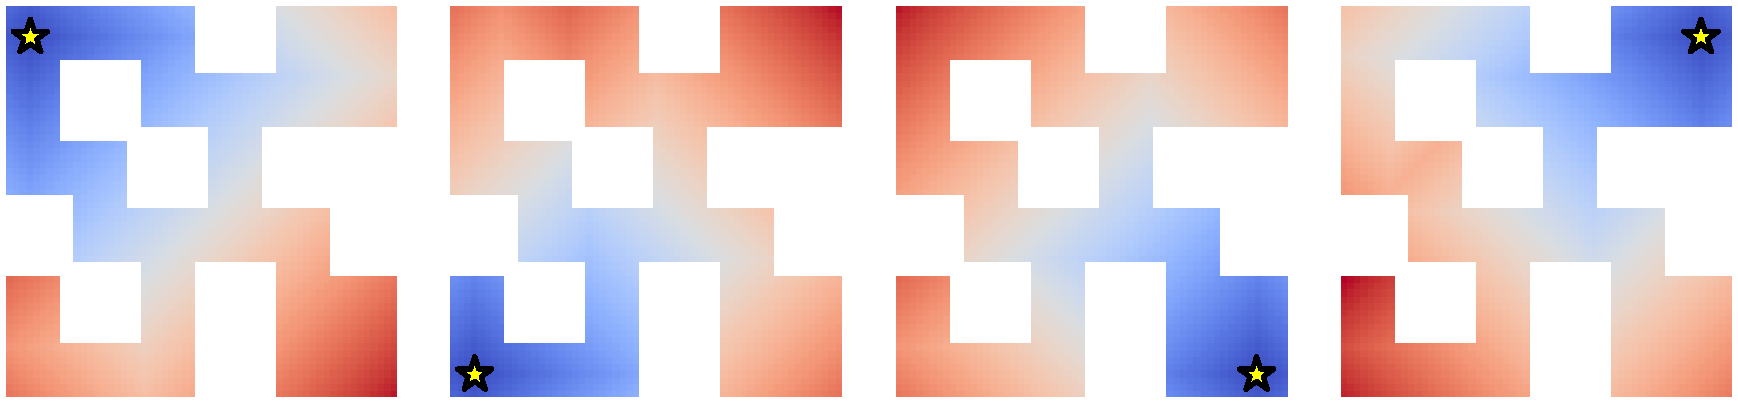
\includegraphics[width=\textwidth]{images/heatmap/medium_geo4_gt.pdf}
        \caption{Ground-Truth using A-star (4 neighbors)}
    \end{subfigure}
    \hfill
    \begin{subfigure}[t]{0.46\textwidth}
        \centering
        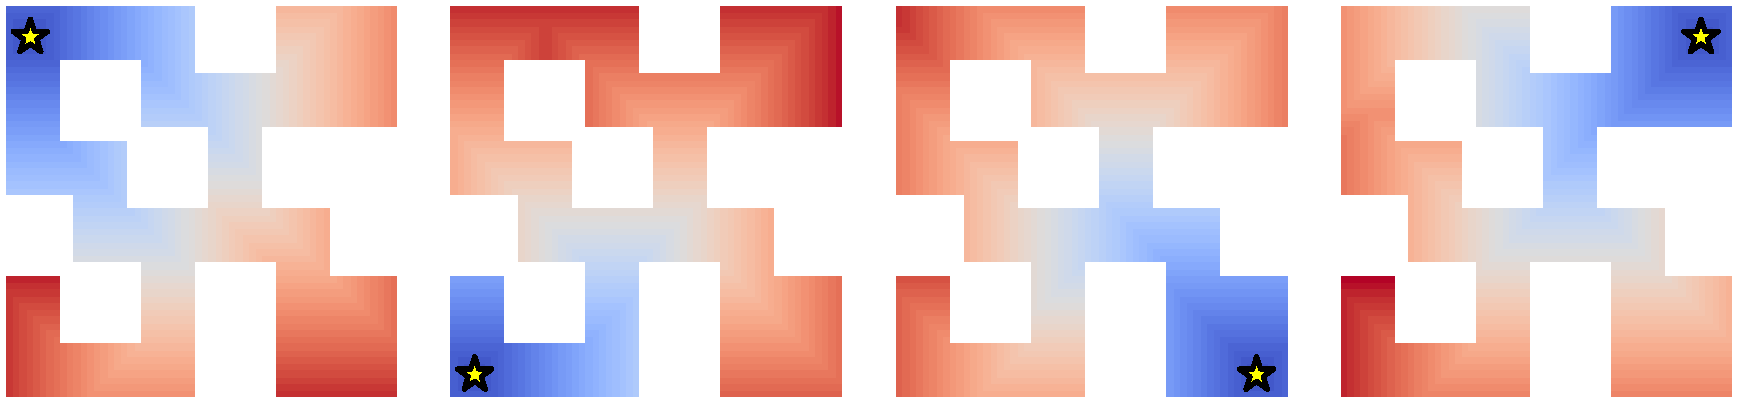
\includegraphics[width=\textwidth]{images/heatmap/medium_geo8_gt.pdf}
        \caption{Ground-Truth using A-star (8 neighbors)}
    \end{subfigure}
    \hfill
    \begin{subfigure}[t]{0.46\textwidth}
        \centering
        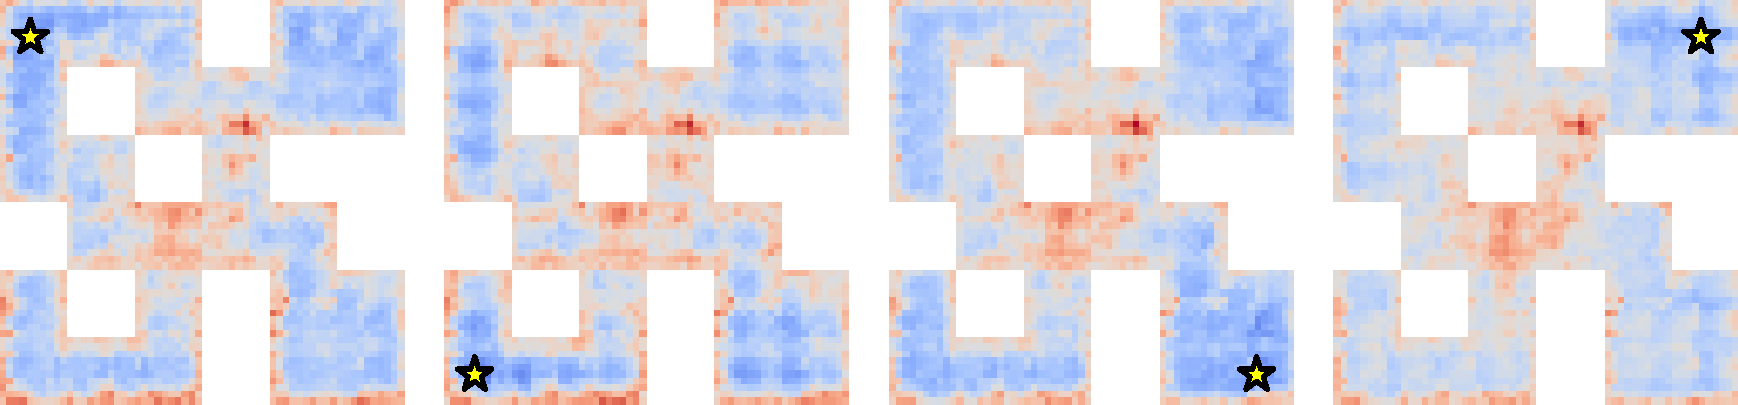
\includegraphics[width=\textwidth]{images/heatmap/medium_dino_cls.pdf}
        \caption{DINOv2 CLS embedding}
    \end{subfigure}
    \hfill
    \begin{subfigure}[t]{0.46\textwidth}
        \centering
        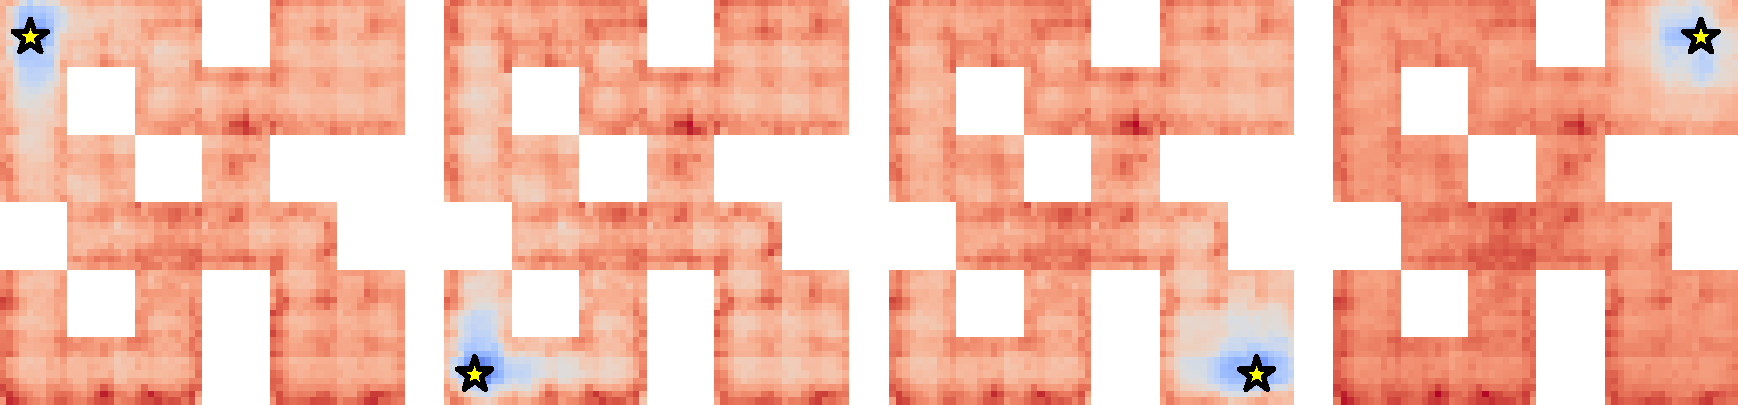
\includegraphics[width=\textwidth]{images/heatmap/medium_dino_patch.pdf}
        \caption{DINOv2 patch embedding}
    \end{subfigure}
    \hfill
    \begin{subfigure}[t]{0.46\textwidth}
        \centering
        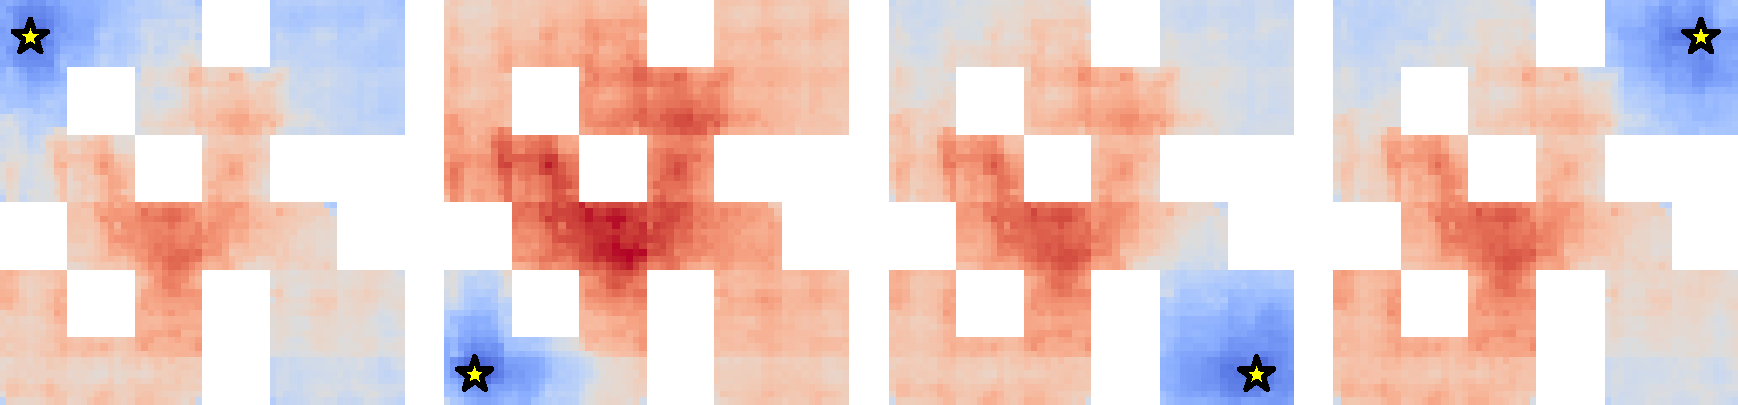
\includegraphics[width=\textwidth]{images/heatmap/proj/medium_False_projchannel_dim8_hw14/patch.pdf}
        \caption{DINOv2 + spatial proj [straightening=False]}
    \end{subfigure}
    \hfill
    \begin{subfigure}[t]{0.46\textwidth}
        \centering
        
\includegraphics[width=\textwidth]{images/heatmap/resnet/medium_False_resnetplus_dim8_hw14_sgTrue_lr1e-5/patch.pdf}
        \caption{ResNet - spatial [straightening=False]}
    \end{subfigure}
    \hfill
    \begin{subfigure}[t]{0.46\textwidth}
        \centering
        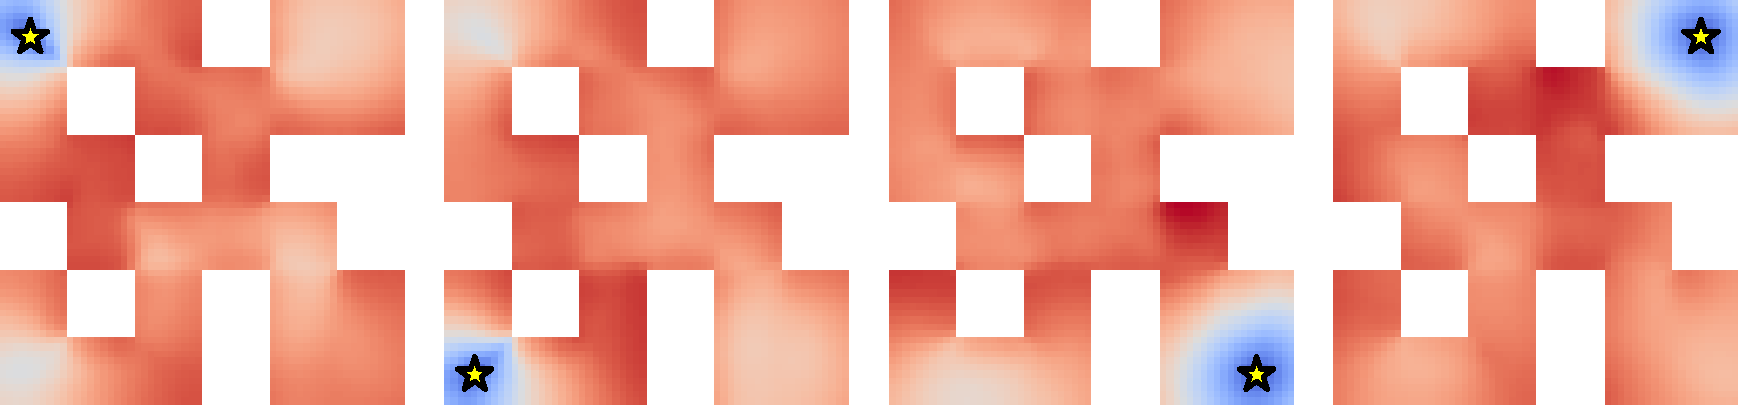
\includegraphics[width=\textwidth]{images/heatmap/resnet/medium_False_resnet_dim384_hw1_sgTrue/global.pdf}
        \caption{ResNet - global [straightening=False]}
    \end{subfigure}
    \hfill
    \begin{subfigure}[t]{0.46\textwidth}
        \centering
        
\includegraphics[width=\textwidth]{images/heatmap/resnet/medium_cos1e-1_resnet_dim384_hw1_sgTrue/global.pdf}
        \caption{ResNet - global [straightening=True]}
    \end{subfigure}
    \hfill
    \begin{subfigure}[t]{0.46\textwidth}
        \centering
        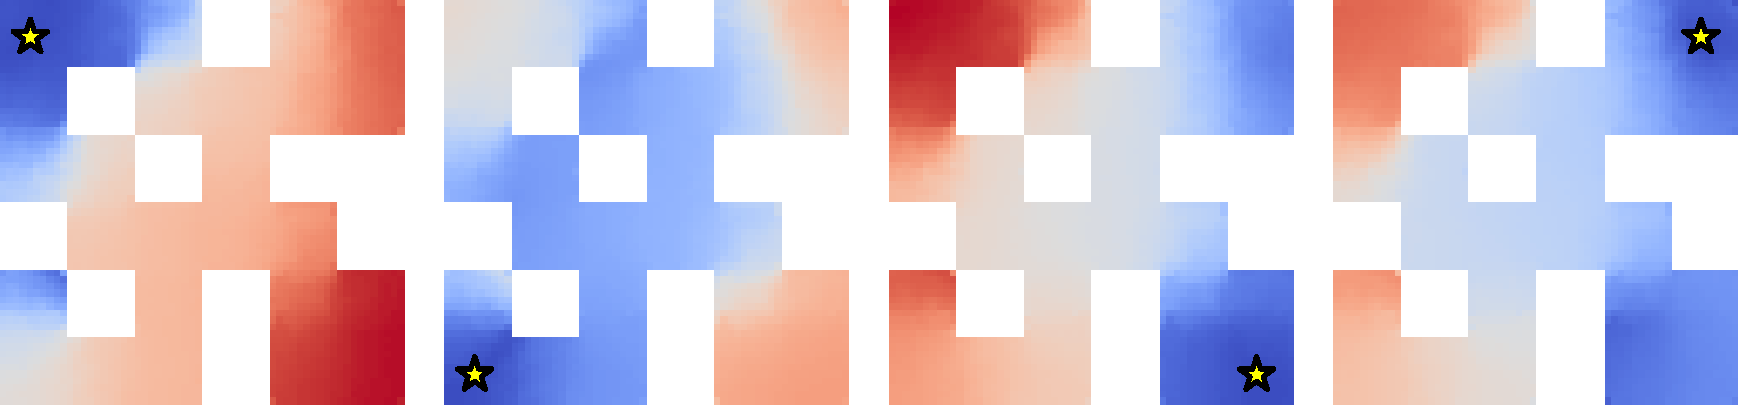
\includegraphics[width=\textwidth]{images/heatmap/proj/medium_aggmlpcos1e-1_projchannel_dim8_hw14/agg.pdf}
        \caption{DINOv2 + spatial proj (agg head) [straightening=True]}
    \end{subfigure}
    \hfill
    \begin{subfigure}[t]{0.46\textwidth}
        \centering
        
\includegraphics[width=\textwidth]{images/heatmap/proj/medium_aggmlpcos1e-1_projchannel_dim8_hw14/patch.pdf}
        \caption{DINOv2 + spatial proj (spatial) [straightening=True]}
    \end{subfigure}
        \begin{subfigure}[t]{0.46\textwidth}
        \centering
        
\includegraphics[width=\textwidth]{images/heatmap/resnet/medium_aggmlpcos1e-1_resnetplus_dim8_hw14/agg.pdf}
        \caption{ResNet - spatial (agg head) [straightening=True]}
    \end{subfigure}
    \hfill
    \begin{subfigure}[t]{0.46\textwidth}
        \centering
        
\includegraphics[width=\textwidth]{images/heatmap/resnet/medium_aggmlpcos1e-1_resnetplus_dim8_hw14/patch.pdf}
        \caption{ResNet - spatial (spatial) [straightening=True]}
    \end{subfigure}
\caption{Distance heatmaps of PointMaze-Medium.
}
\label{img:more_heatmap_medium}
\end{figure}

\clearpage

\subsection{Visualization of Latent Trajectories}
\label{app:pca}
To visualize the learned representations of the trajectories, we randomly sample trajectories with a length of 30 and plot them in 2D using PCA. Here, we use DINO CLS token embeddings and the aggregated features of our model (trained with straightening). While latent trajectories are highly curved in DINO CLS embedding space, they become significantly smoother after straightening. Additionally, we compute the MSE between the embeddings of each intermediate state and the target. The Euclidean distance is closer to the geodesic distance for straighter trajectories, and thus MSE (which is squared Euclidean distance) becomes a more useful planning cost function that can reflect the true progress towards the target. Visualizations for different environments are in~\Cref{img:more_pca_wall,img:more_pca_umaze,img:more_pca_medium,img:more_pca_pusht}.

\begin{figure*}[h]
    \centering
    \begin{subfigure}[t]{\textwidth}
        \centering
        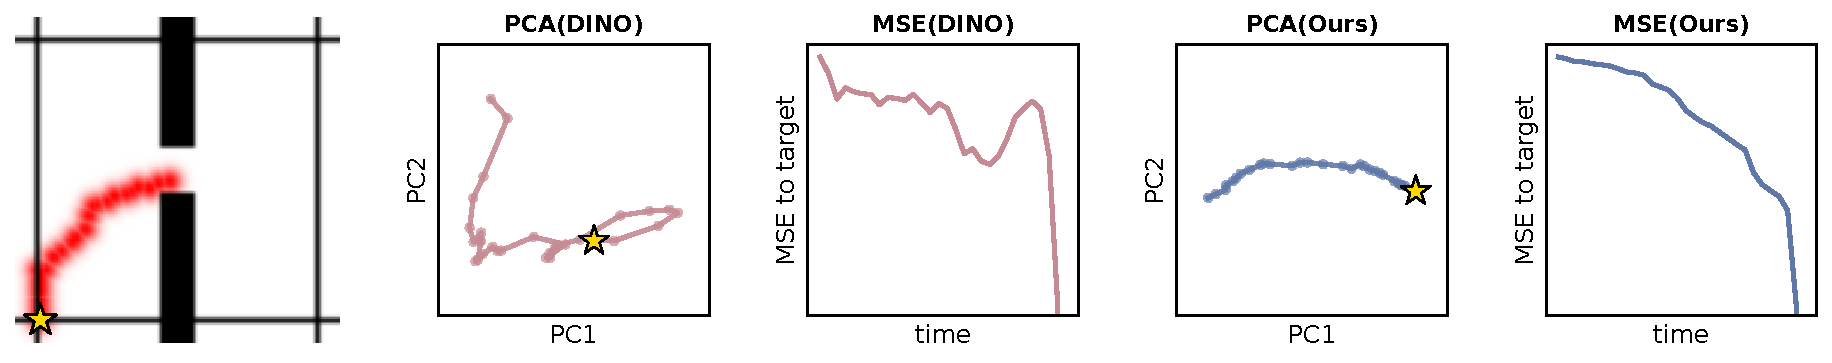
\includegraphics[width=0.95\textwidth]{images/wall_exp2_pca_mse.pdf}
    \end{subfigure}
    \begin{subfigure}[t]{\textwidth}
    \centering
    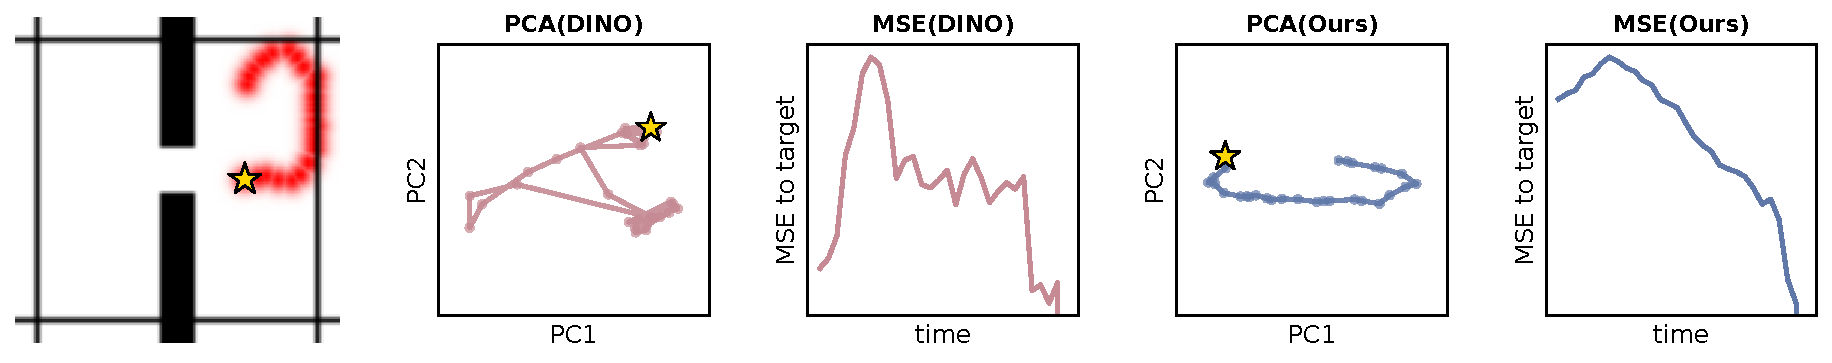
\includegraphics[width=0.95\textwidth]{images/wall_exp3_pca_mse.pdf}
    \end{subfigure}
\caption{PCA of Trajectories of Wall.}
\label{img:more_pca_wall}
\end{figure*}

\begin{figure*}[h]
    \centering
    \begin{subfigure}[t]{\textwidth}
        \centering
        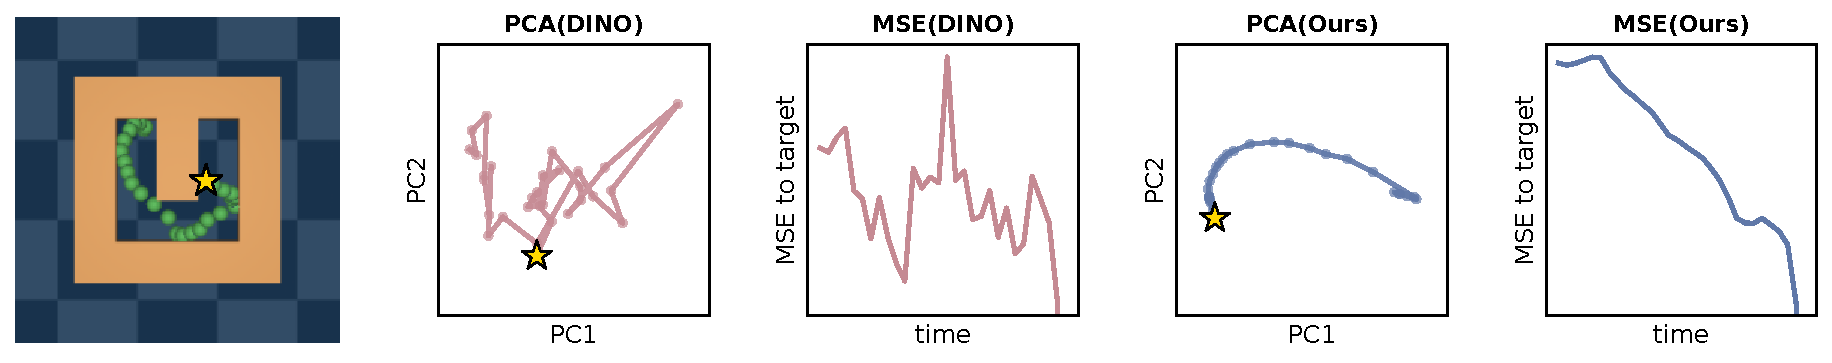
\includegraphics[width=0.95\textwidth]{images/umaze_exp2_pca_mse.pdf}
    \end{subfigure}
    \begin{subfigure}[t]{\textwidth}
    \centering
    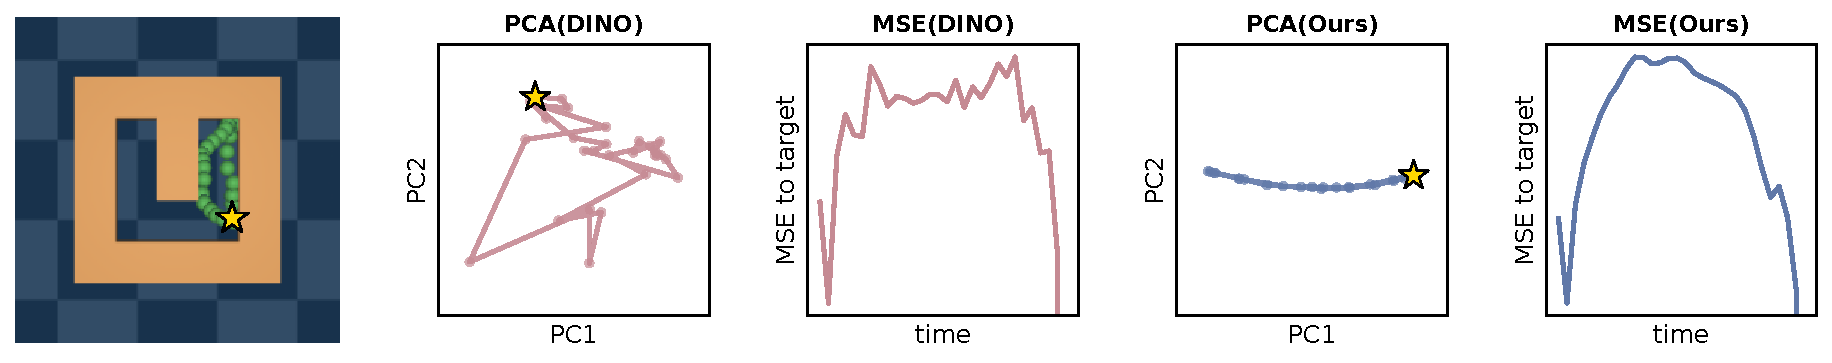
\includegraphics[width=0.95\textwidth]{images/umaze_exp3_pca_mse.pdf}
    \end{subfigure}
\caption{PCA of Trajectories of PointMaze-UMaze.}
\label{img:more_pca_umaze}
\end{figure*}

\begin{figure*}[h]
    \centering
    \begin{subfigure}[t]{\textwidth}
        \centering
        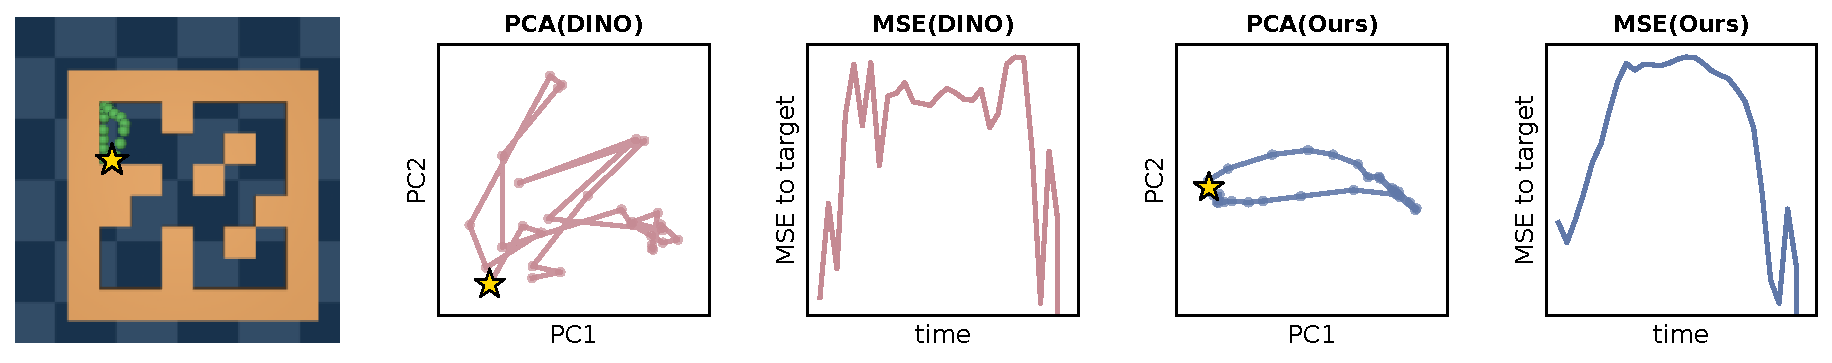
\includegraphics[width=0.95\textwidth]{images/medium_exp1_pca_mse.pdf}
    \end{subfigure}
    \begin{subfigure}[t]{\textwidth}
        \centering
        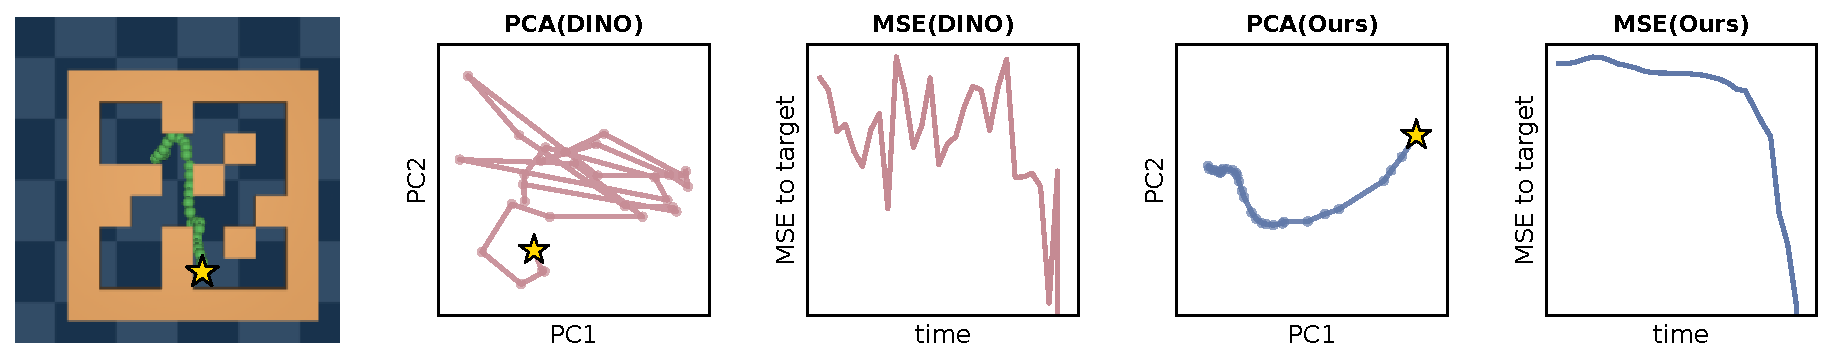
\includegraphics[width=0.95\textwidth]{images/medium_exp2_pca_mse.pdf}
    \end{subfigure}
    \begin{subfigure}[t]{\textwidth}
    \centering
    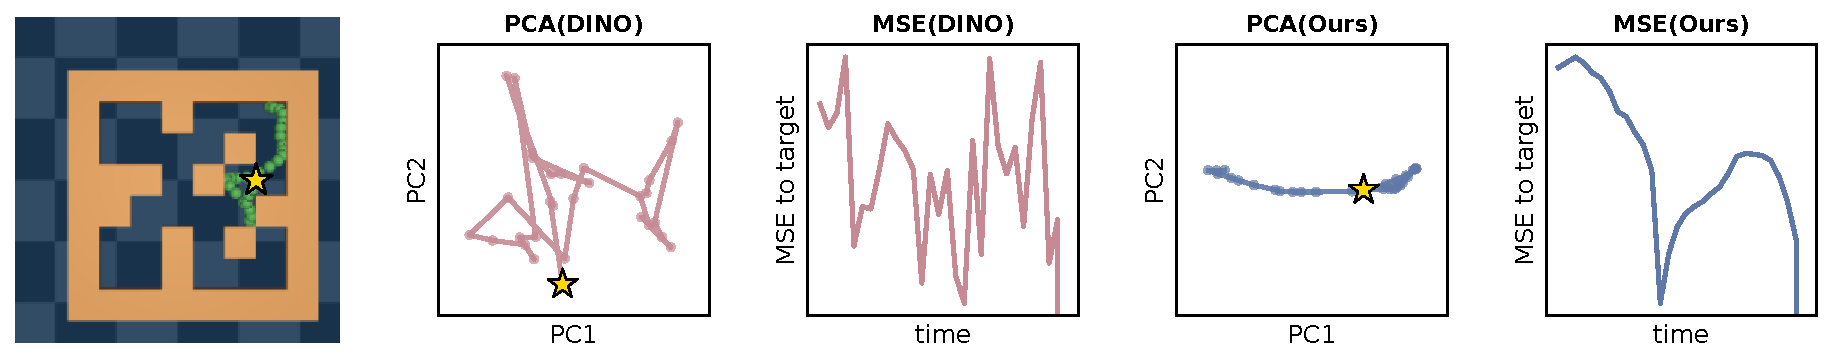
\includegraphics[width=0.95\textwidth]{images/medium_exp3_pca_mse.pdf}
    \end{subfigure}
\caption{PCA of Trajectories of PointMaze-Medium.}
\label{img:more_pca_medium}
\end{figure*}

\begin{figure*}[h]
    \centering
    \begin{subfigure}[t]{\textwidth}
        \centering
        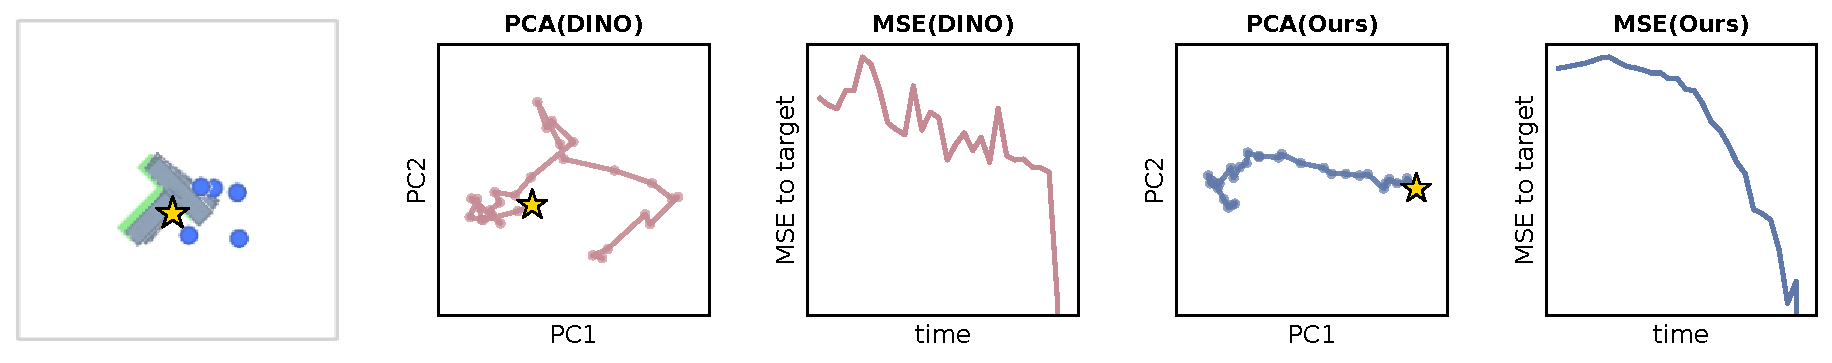
\includegraphics[width=0.95\textwidth]{images/pusht_exp1_pca_mse.pdf}
    \end{subfigure}
    \begin{subfigure}[t]{\textwidth}
        \centering
        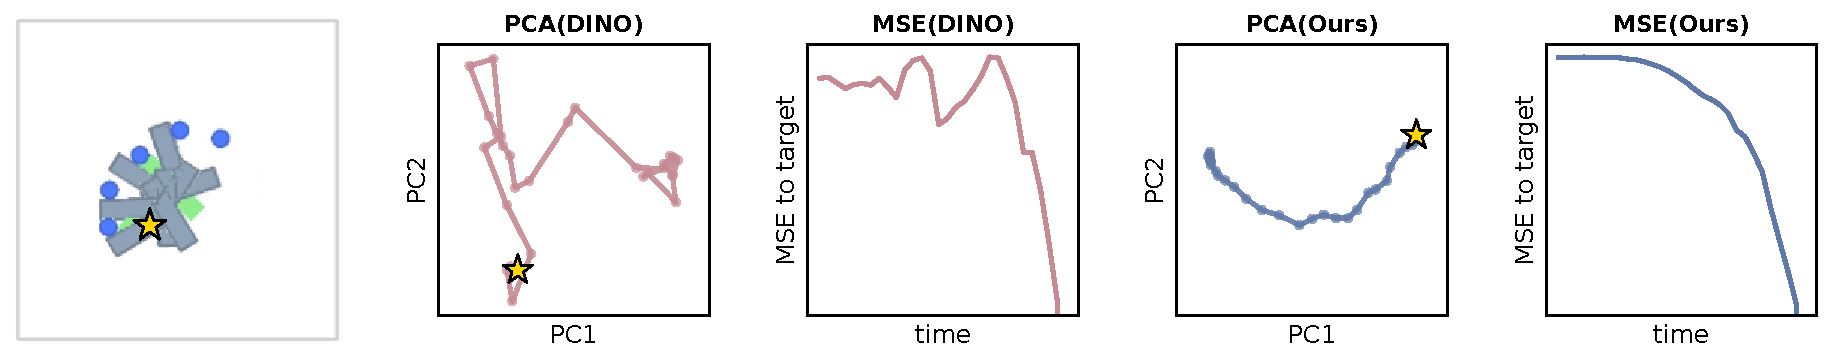
\includegraphics[width=0.95\textwidth]{images/pusht_exp2_pca_mse.pdf}
    \end{subfigure}
    \begin{subfigure}[t]{\textwidth}
    \centering
    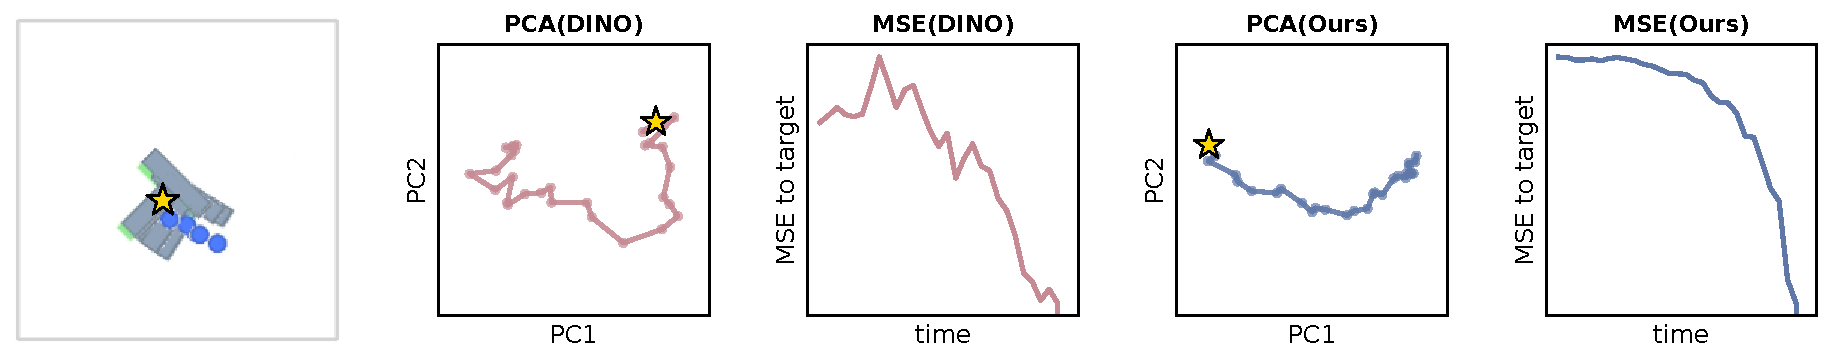
\includegraphics[width=0.95\textwidth]{images/pusht_exp3_pca_mse.pdf}
    \end{subfigure}
\caption{PCA of Trajectories of PushT. The overlaid figures only include five samples for readability.}
\label{img:more_pca_pusht}
\end{figure*}

\clearpage

\subsection{Planning Trajectories}
\label{app:traj}

\begin{figure}[h]
    \centering
    \begin{subfigure}[t]{\textwidth}
        \centering
        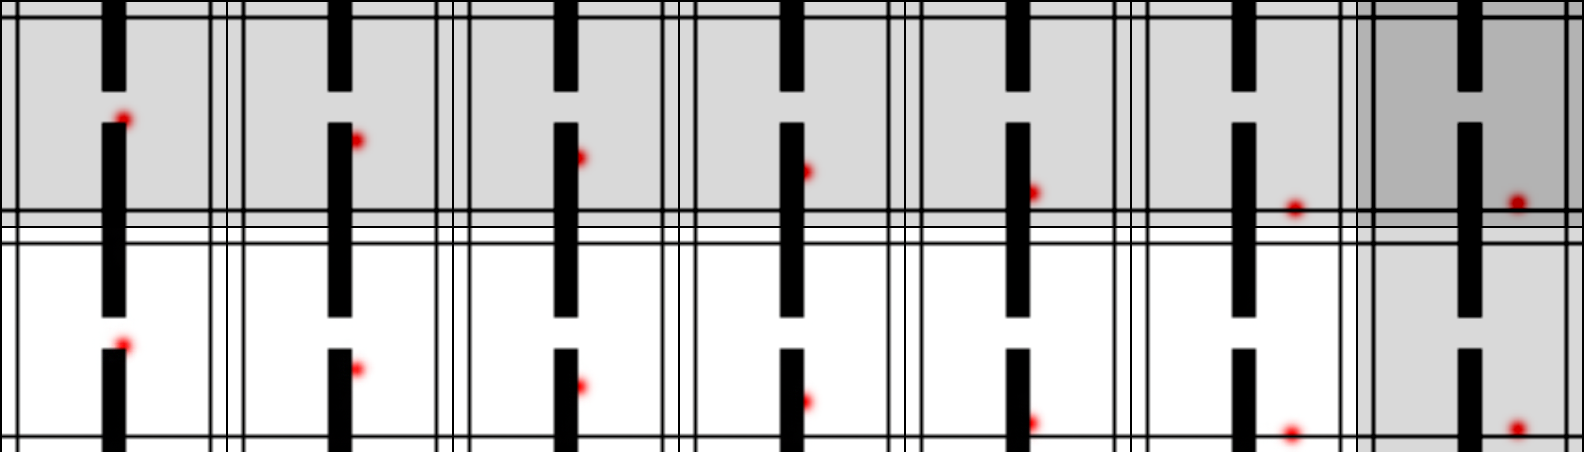
\includegraphics[width=0.95\textwidth]{images/wall_exp1.png}
        \vspace{0.1in}
    \end{subfigure}
    \begin{subfigure}[t]{\textwidth}
        \centering
        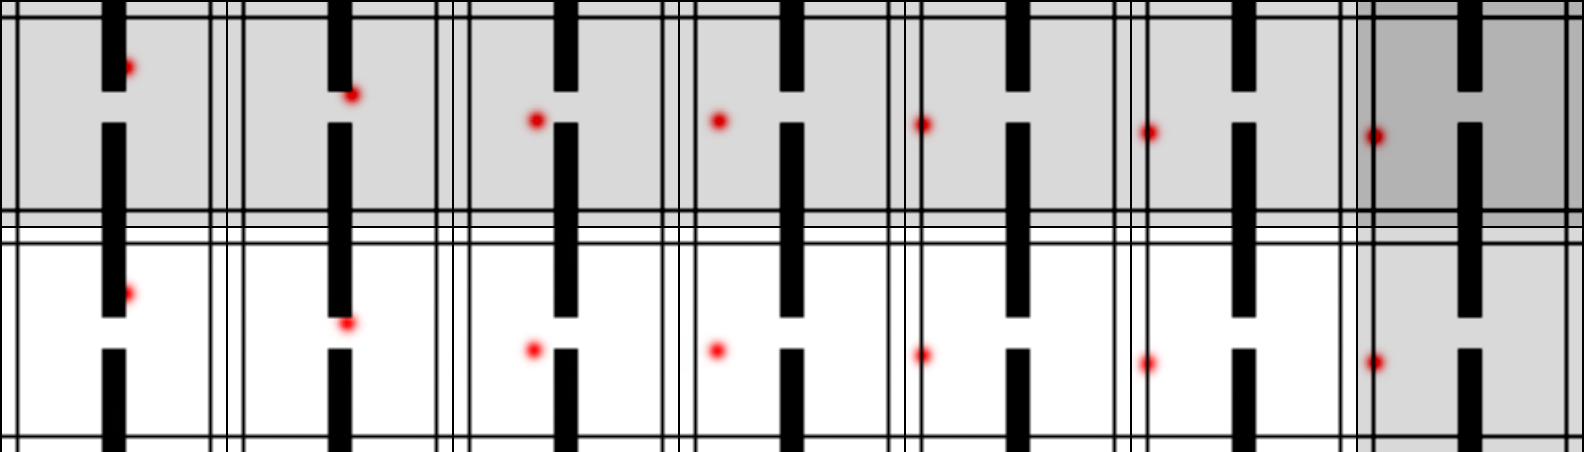
\includegraphics[width=0.95\textwidth]{images/wall_exp2.png}
        \vspace{0.1in}
    \end{subfigure}
    \begin{subfigure}[t]{\textwidth}
        \centering
        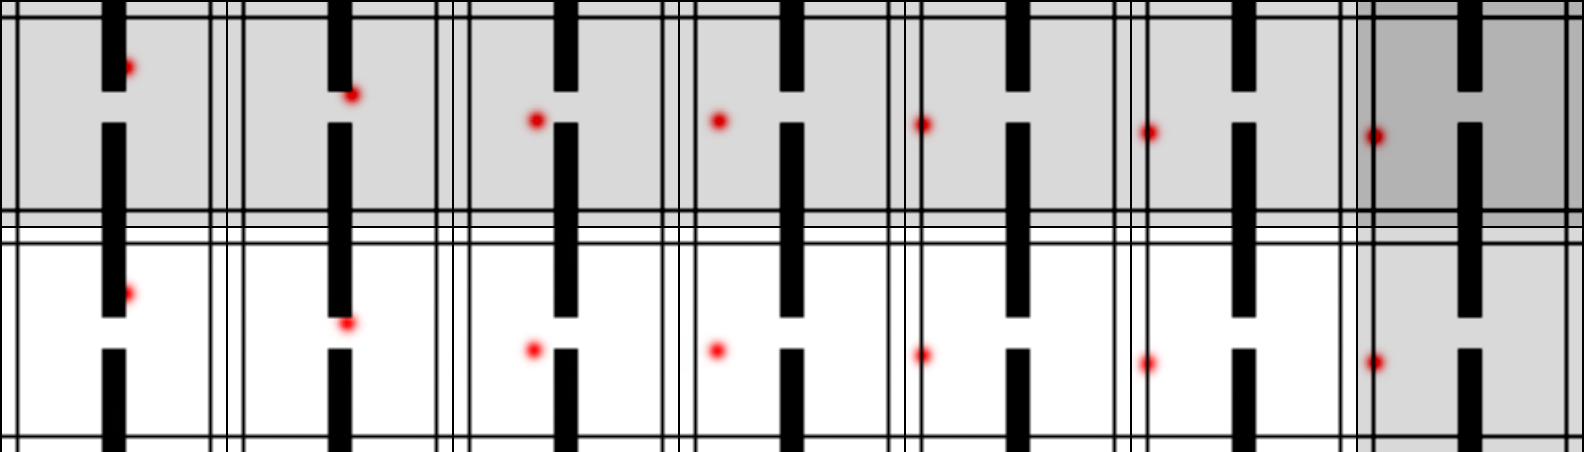
\includegraphics[width=0.95\textwidth]{images/wall_exp3.png}
        \vspace{0.1in}
    \end{subfigure}
\caption{Open-Loop Planning Trajectories of Wall. The first row is from the simulator and the second from the decoder. The last column is the goal image.}
\label{img:plan_traj_pusht}
\end{figure}

\begin{figure*}[h]
    \centering
    \begin{subfigure}[t]{\textwidth}
        \centering
        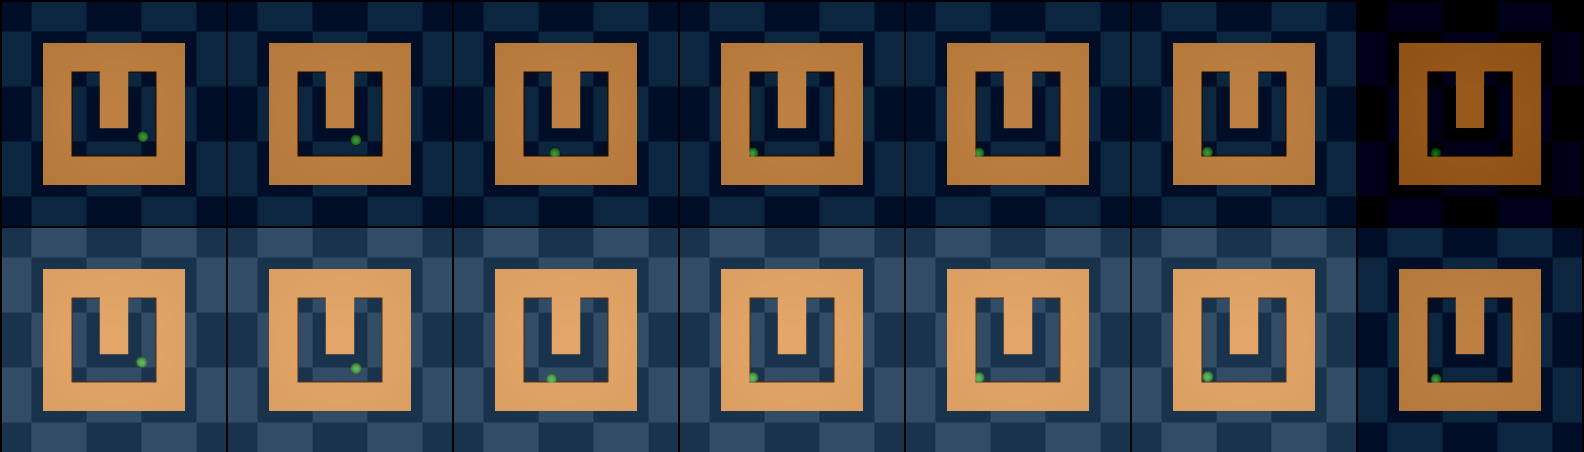
\includegraphics[width=0.95\textwidth]{images/umaze_exp1.png}
        \vspace{0.1in}
    \end{subfigure}
    \begin{subfigure}[t]{\textwidth}
        \centering
        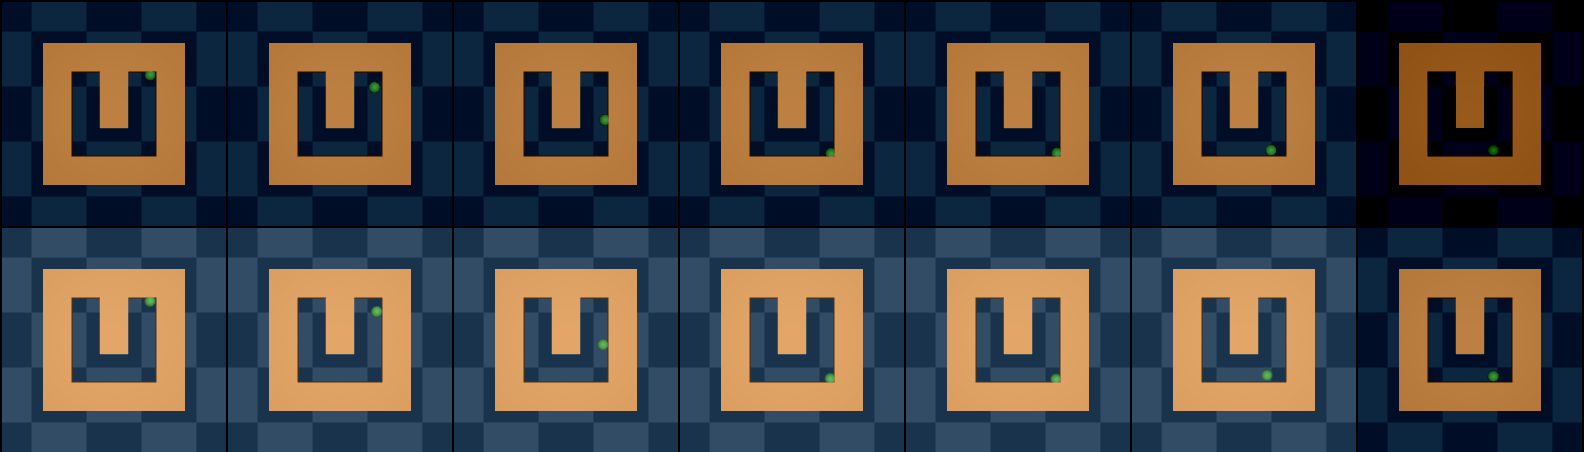
\includegraphics[width=0.95\textwidth]{images/umaze_exp2.png}
        \vspace{0.1in}
    \end{subfigure}
    \begin{subfigure}[t]{\textwidth}
        \centering
        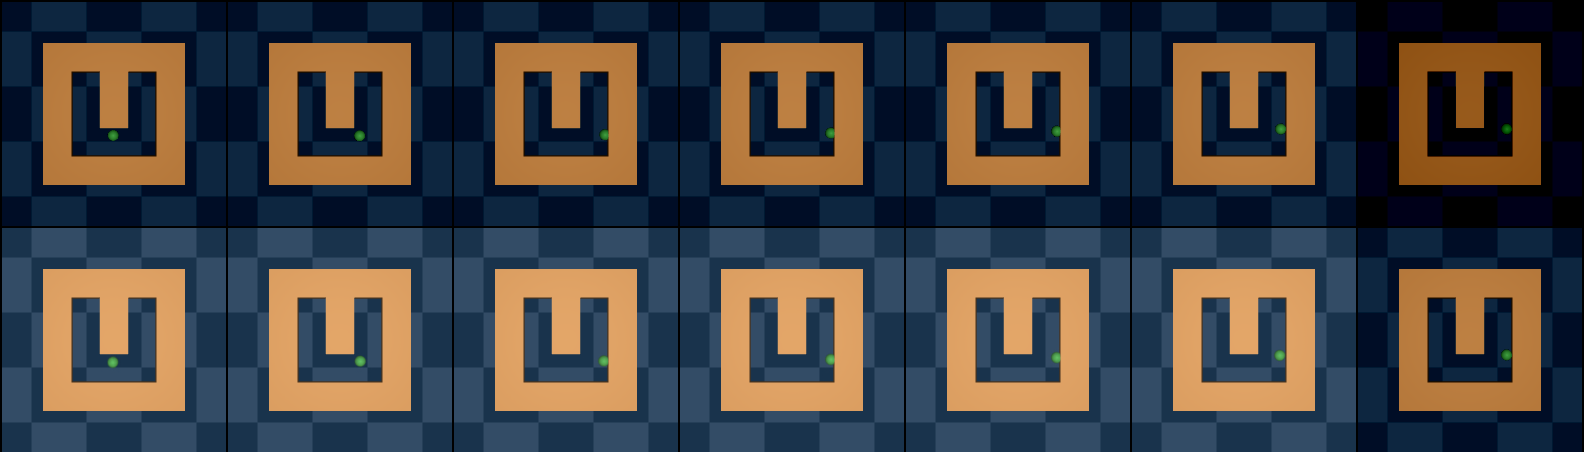
\includegraphics[width=0.95\textwidth]{images/umaze_exp3.png}
        \vspace{0.1in}
    \end{subfigure}
    \begin{subfigure}[t]{\textwidth}
        \centering
        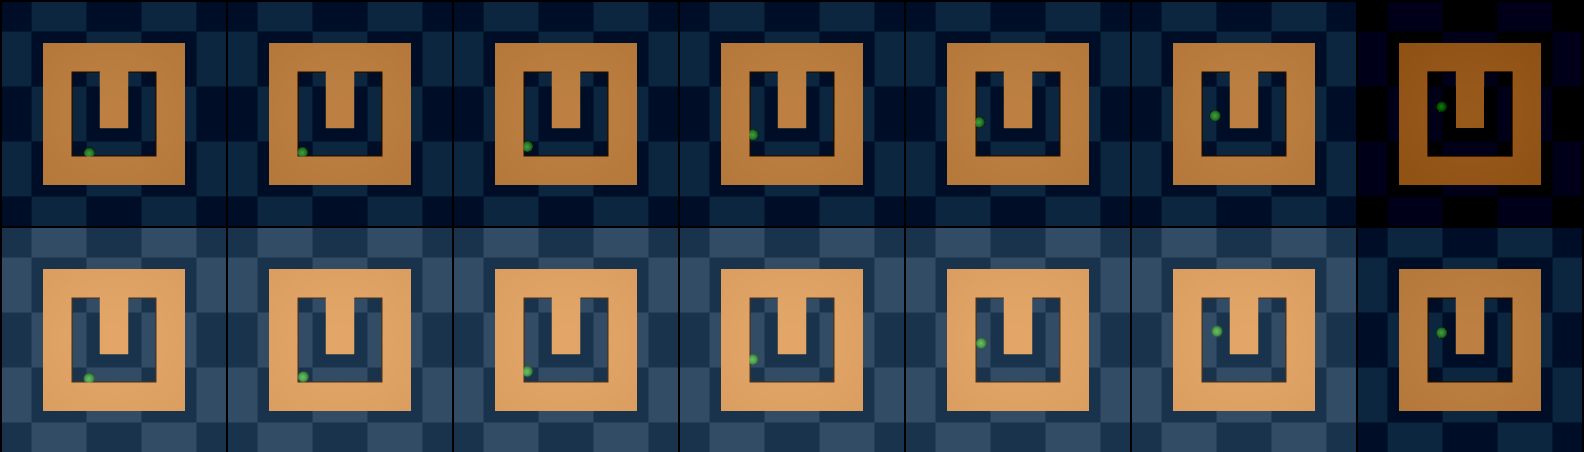
\includegraphics[width=0.95\textwidth]{images/umaze_exp4.png}
    \end{subfigure}
\caption{Open-Loop Planning Trajectories of PointMaze-UMaze. The first row is from the simulator and the second from the decoder. The last column is the goal image.}
\label{img:plan_traj_umaze}
\end{figure*}

\begin{figure*}[h]
    \centering
    \begin{subfigure}[t]{\textwidth}
        \centering
        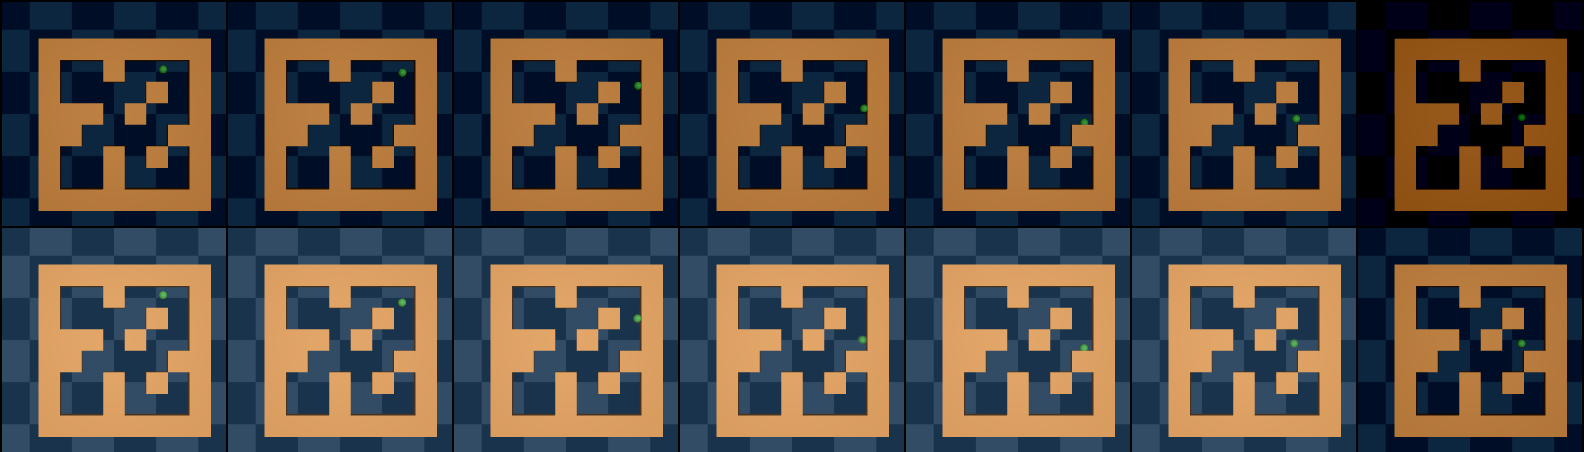
\includegraphics[width=0.95\textwidth]{images/medium_exp1.png}
        \vspace{0.1in}
    \end{subfigure}
    \begin{subfigure}[t]{\textwidth}
        \centering
        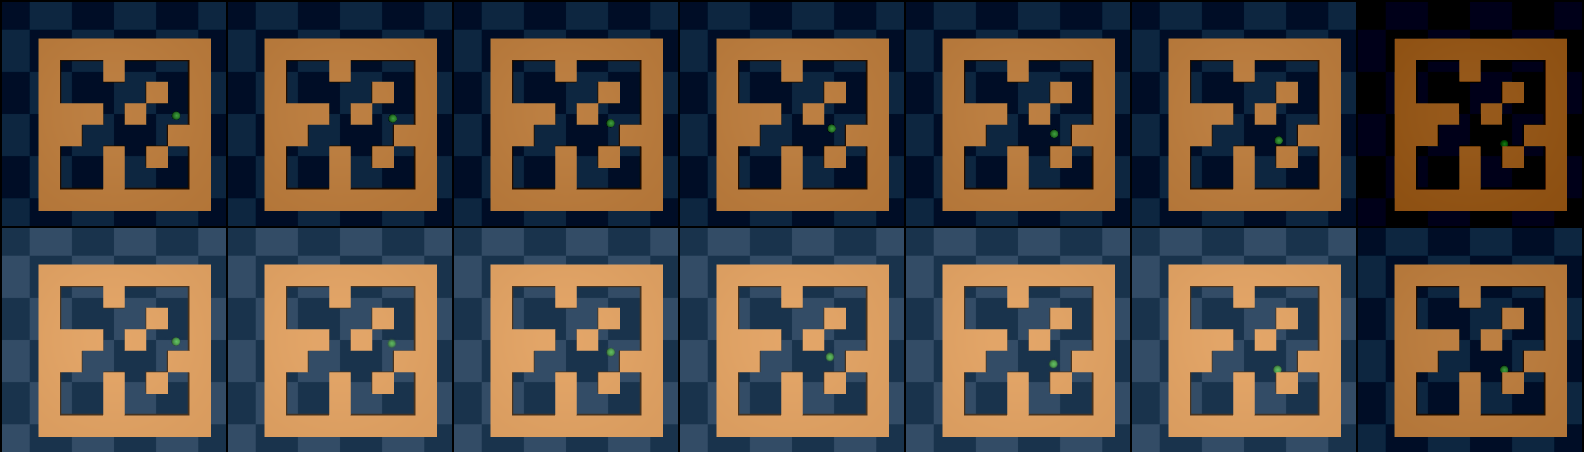
\includegraphics[width=0.95\textwidth]{images/medium_exp2.png}
        \vspace{0.1in}
    \end{subfigure}
    \begin{subfigure}[t]{\textwidth}
        \centering
        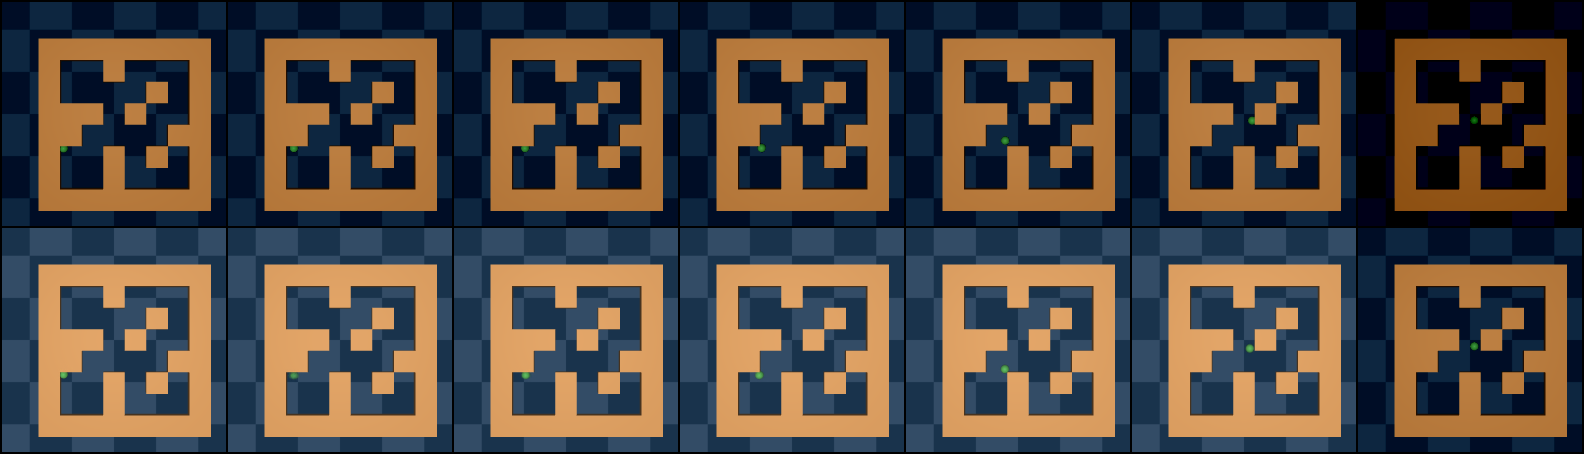
\includegraphics[width=0.95\textwidth]{images/medium_exp3.png}
        \vspace{0.1in}
    \end{subfigure}
    \begin{subfigure}[t]{\textwidth}
        \centering
        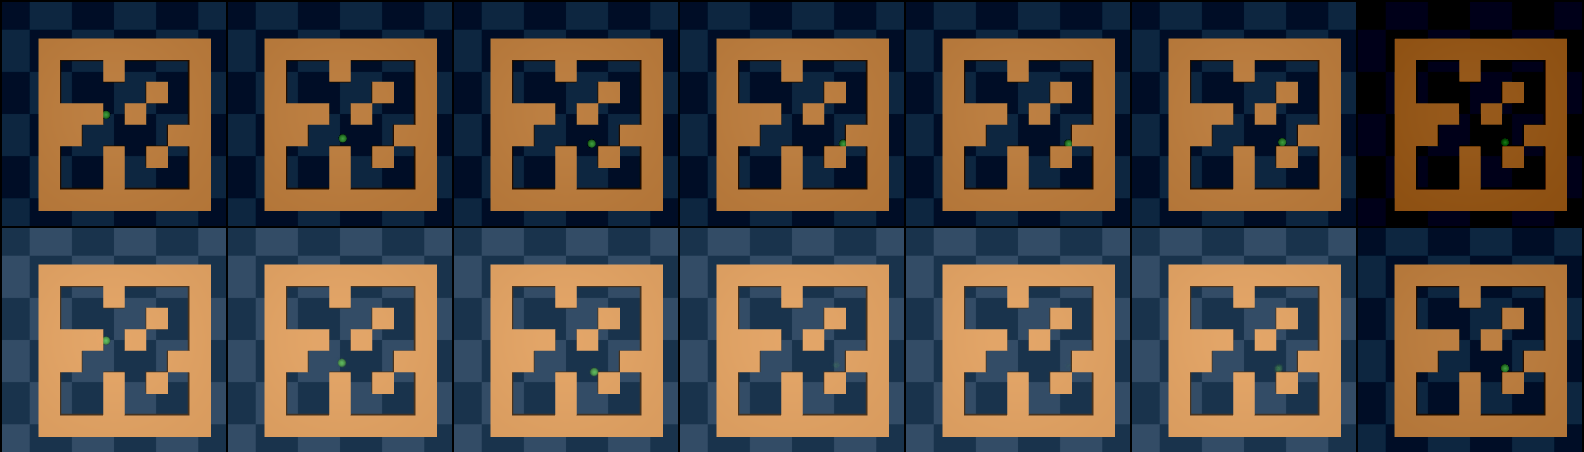
\includegraphics[width=0.95\textwidth]{images/medium_exp4.png}
    \end{subfigure}
\caption{Open-Loop Planning Trajectories of PointMaze-Medium. The first row is from the simulator and the second from the decoder. The last column is the goal image.}
\label{img:plan_traj_medium}
\end{figure*}

\begin{figure*}[h]
    \centering
    \begin{subfigure}[t]{\textwidth}
        \centering
        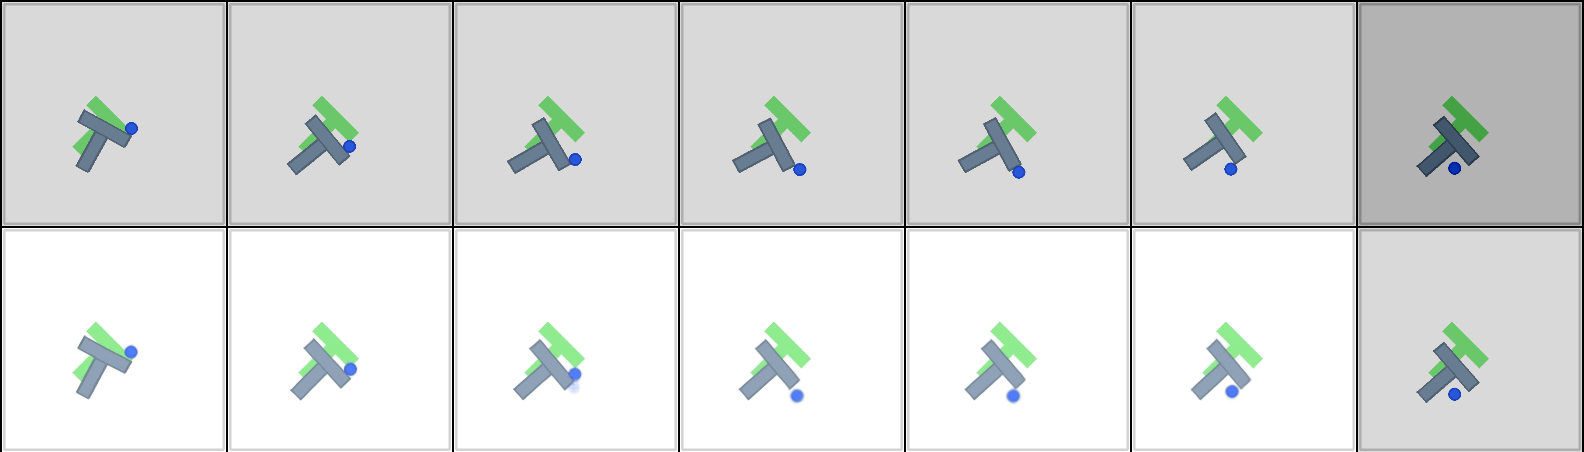
\includegraphics[width=0.95\textwidth]{images/pusht_exp1.png}
        \vspace{0.1in}
    \end{subfigure}
    \begin{subfigure}[t]{\textwidth}
        \centering
        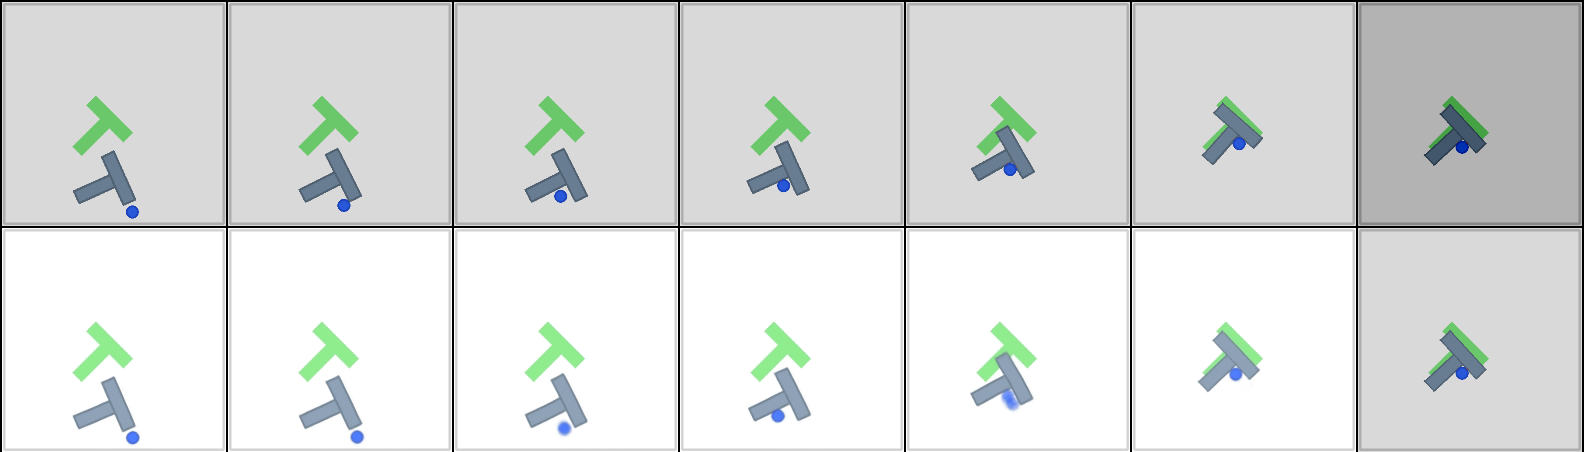
\includegraphics[width=0.95\textwidth]{images/pusht_exp2.png}
        \vspace{0.1in}
    \end{subfigure}
    \begin{subfigure}[t]{\textwidth}
        \centering
        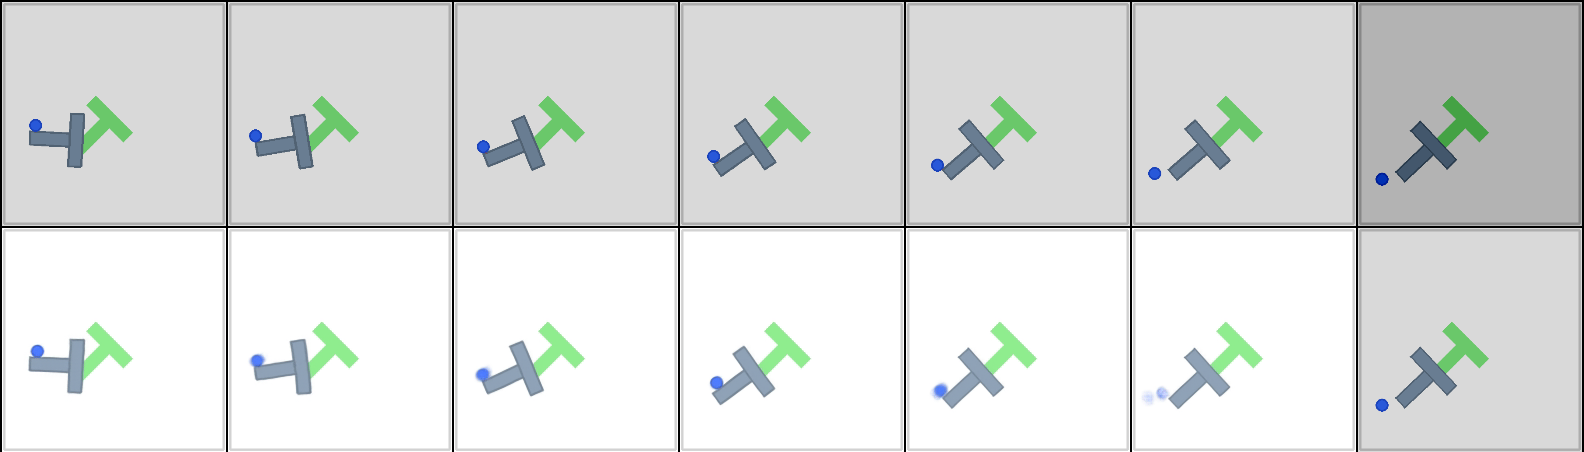
\includegraphics[width=0.95\textwidth]{images/pusht_exp3.png}
        \vspace{0.1in}
    \end{subfigure}
    \begin{subfigure}[t]{\textwidth}
        \centering
        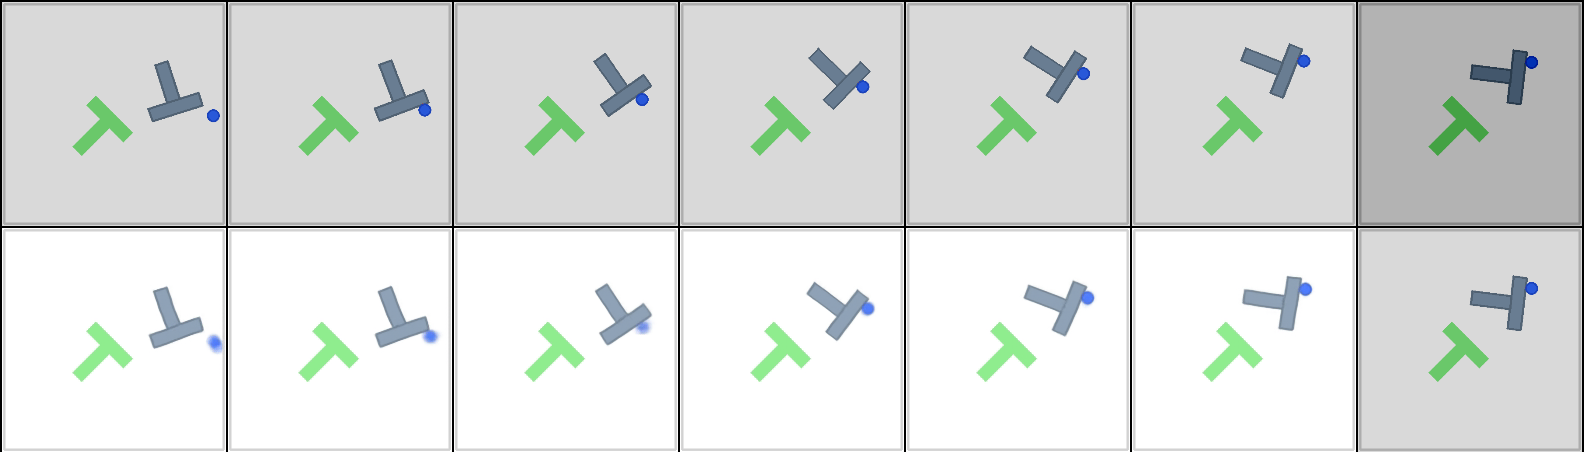
\includegraphics[width=0.95\textwidth]{images/pusht_exp4.png}
    \end{subfigure}
\caption{Open-Loop Planning Trajectories of PushT. The first row is from the simulator and the second from the decoder.}
\label{img:plan_traj_pusht}
\end{figure*}

\clearpage
\section{Teleported-PointMaze}
\label{appendix:teleportation}

This is a novel 2D navigation environment adapted from PointMaze. The core modification is a one-way teleportation dynamic. While the top, bottom, and left boundaries of the maze function as standard solid obstacles, a predefined region near the right wall acts as a teleportation trigger. If an agent's state transition at time $t$ results in a new x-position $x_{t+1}$ that crosses this threshold (i.e., $x_{t+1} > x_{\text{right-border}}$), an instantaneous state intervention occurs, modifying the agent's state as follows:

\begin{enumerate}
    \item Position (x): The agent's x-position is reset to the left side of the maze: $x_{t+1} \leftarrow x_{\text{left-border}}$.
    \item Position (y): The agent's y-position $y_{t+1}$ is preserved.
    \item Velocity (x): The agent's x-axis velocity $v_x$ is reset to its absolute value: $v_{x, t+1} \leftarrow |v_{x, t}|$.
\end{enumerate}

\begin{figure*}[h]
\center
\includegraphics[width=\textwidth]{images/example_teleport.pdf}
\caption{Teleported-PointMaze. Note that the teleportation happens inside the red box.
}
\label{img:teleport}
\end{figure*}

\begin{figure*}[h]
\center
    \begin{subfigure}[t]{0.46\textwidth}
        \centering
        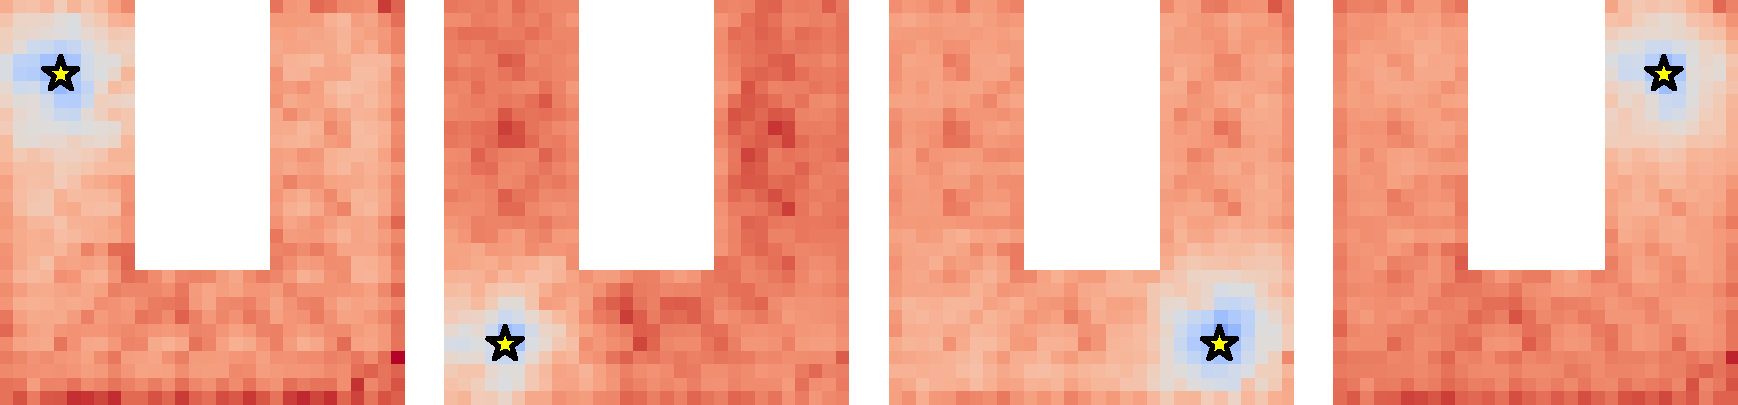
\includegraphics[width=\textwidth]{images/heatmap/umaze_dino_patch.pdf}
        \caption{DINOv2 patch embedding}
    \end{subfigure}
    \hfill
    \begin{subfigure}[t]{0.46\textwidth}
        \centering
        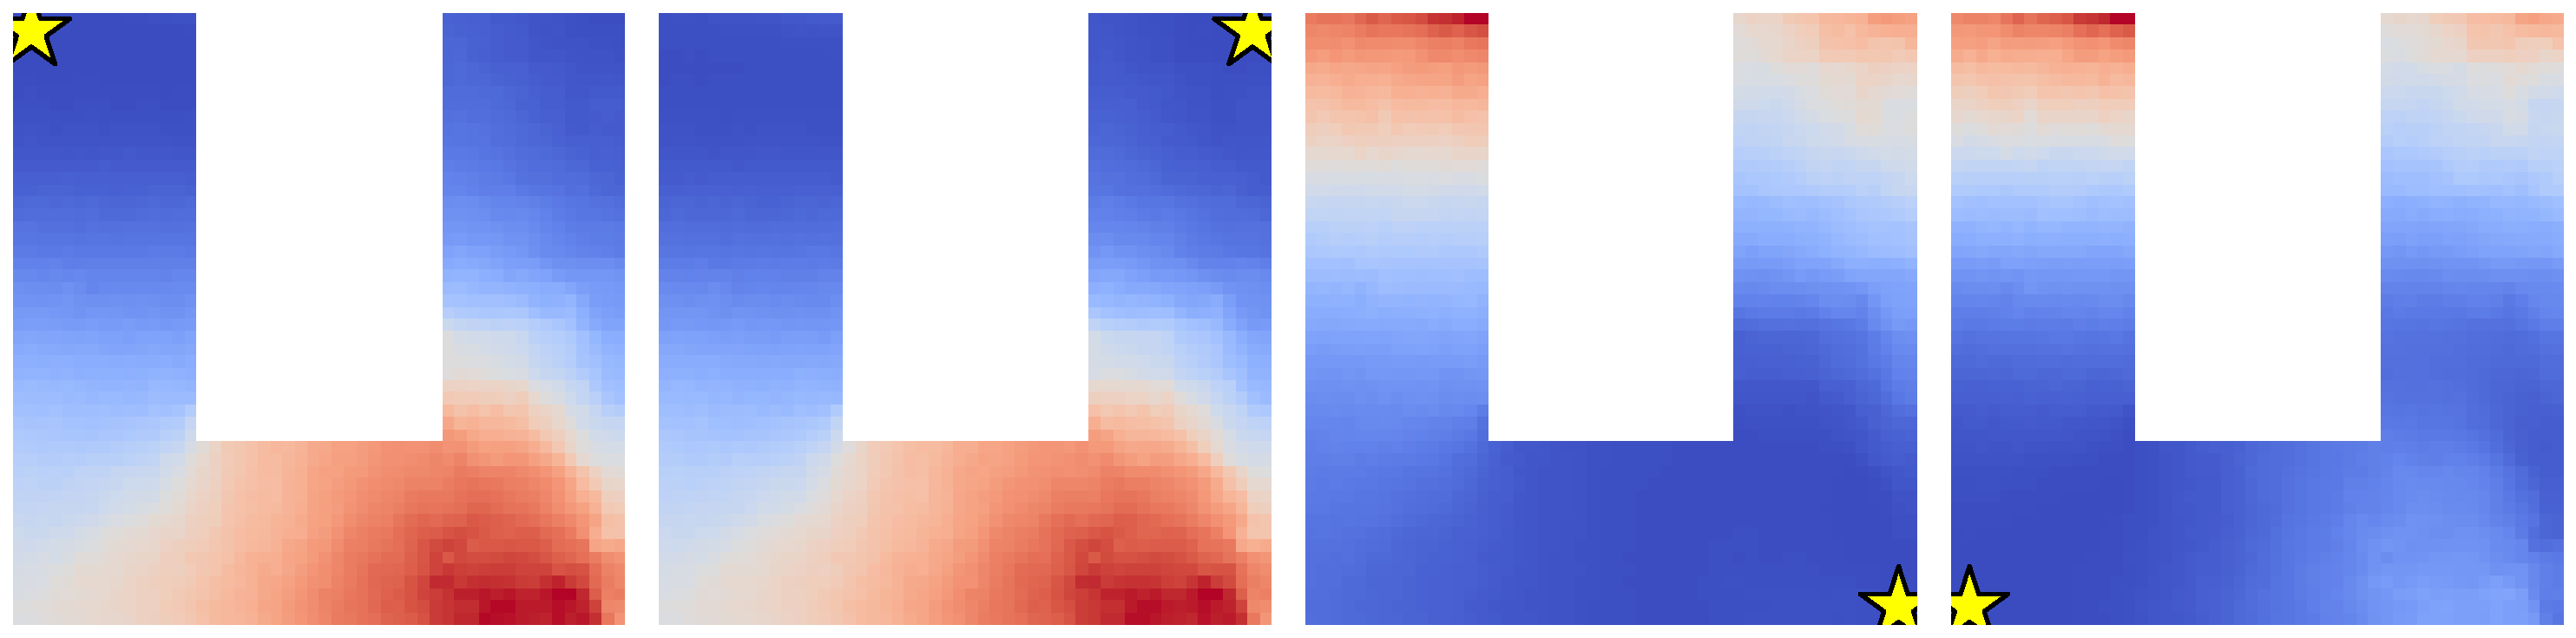
\includegraphics[width=\textwidth]{images/heatmap/heatmap_teleport_strcos.pdf}
        \caption{Trained projector with straightening}
    \end{subfigure}
    \hfill
    \begin{subfigure}[t]{0.46\textwidth}
        \centering
        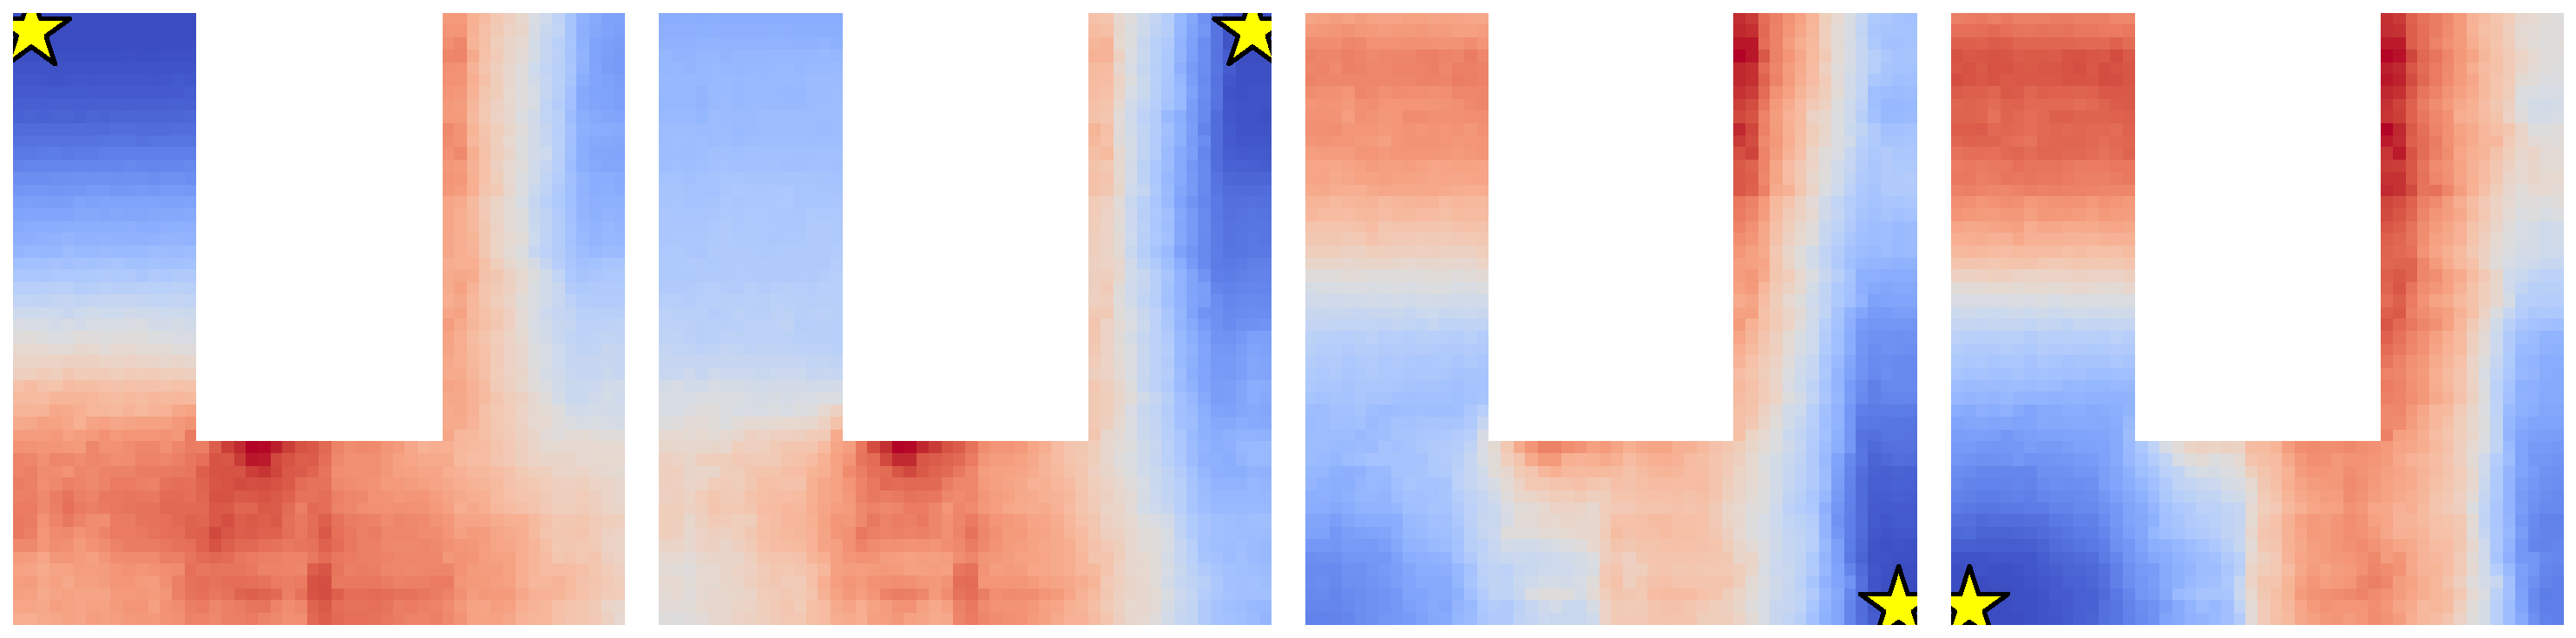
\includegraphics[width=\textwidth]{images/heatmap/heatmap_teleport_strFalse.pdf}
        \caption{Trained projector without straightening}
    \end{subfigure}
    \hfill
    \begin{subfigure}[t]{0.46\textwidth}
        \centering
        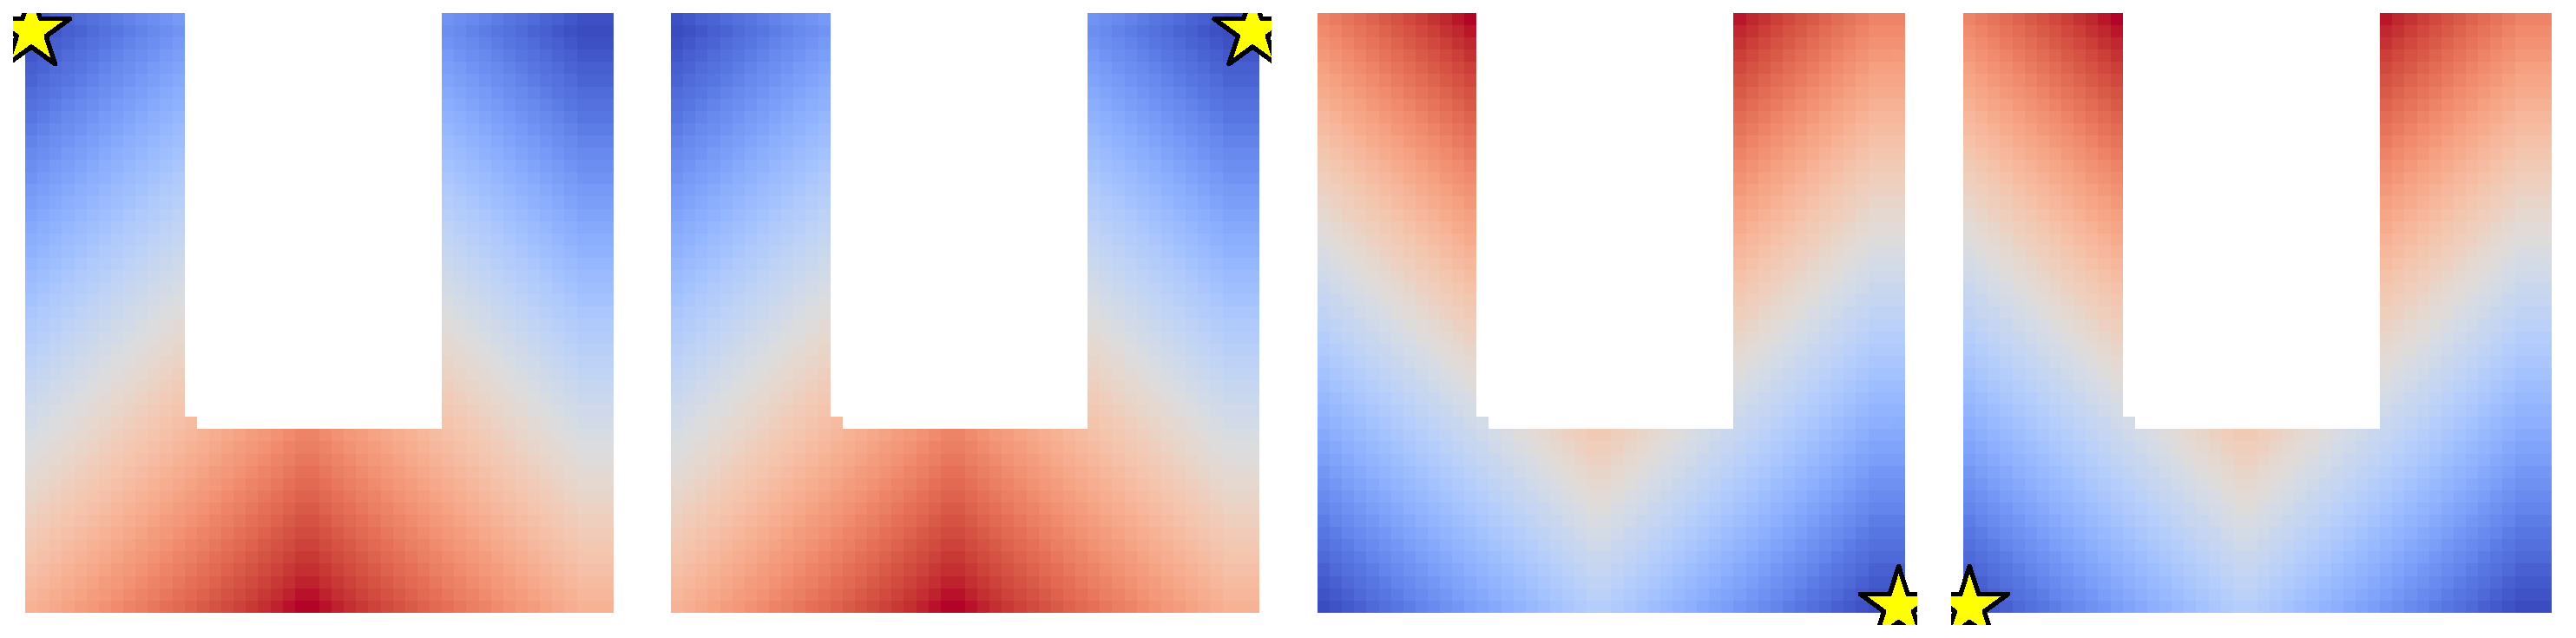
\includegraphics[width=\textwidth]{images/heatmap/heatmap_teleport_gt.pdf}
        \caption{Ground-Truth using A-star}
    \end{subfigure}
\caption{Distance heatmaps of Teleported-PointMaze (blue indicates small values, red indicates large values). The state marked by the yellow star is used as the target, and we compute the MSE between its embedding and those of all other states in the maze. Since MSE is symmetric, this visualization does not fully capture directional reachability in the asymmetric teleportation dynamics. Nevertheless, with straightening, the resulting heatmaps are significantly closer to the transition-aware distances obtained using A-star.}
\label{img:heatmap_teleport}
\end{figure*}

\begin{figure*}[h]
\center
    \begin{subfigure}[t]{\textwidth}
        \centering
        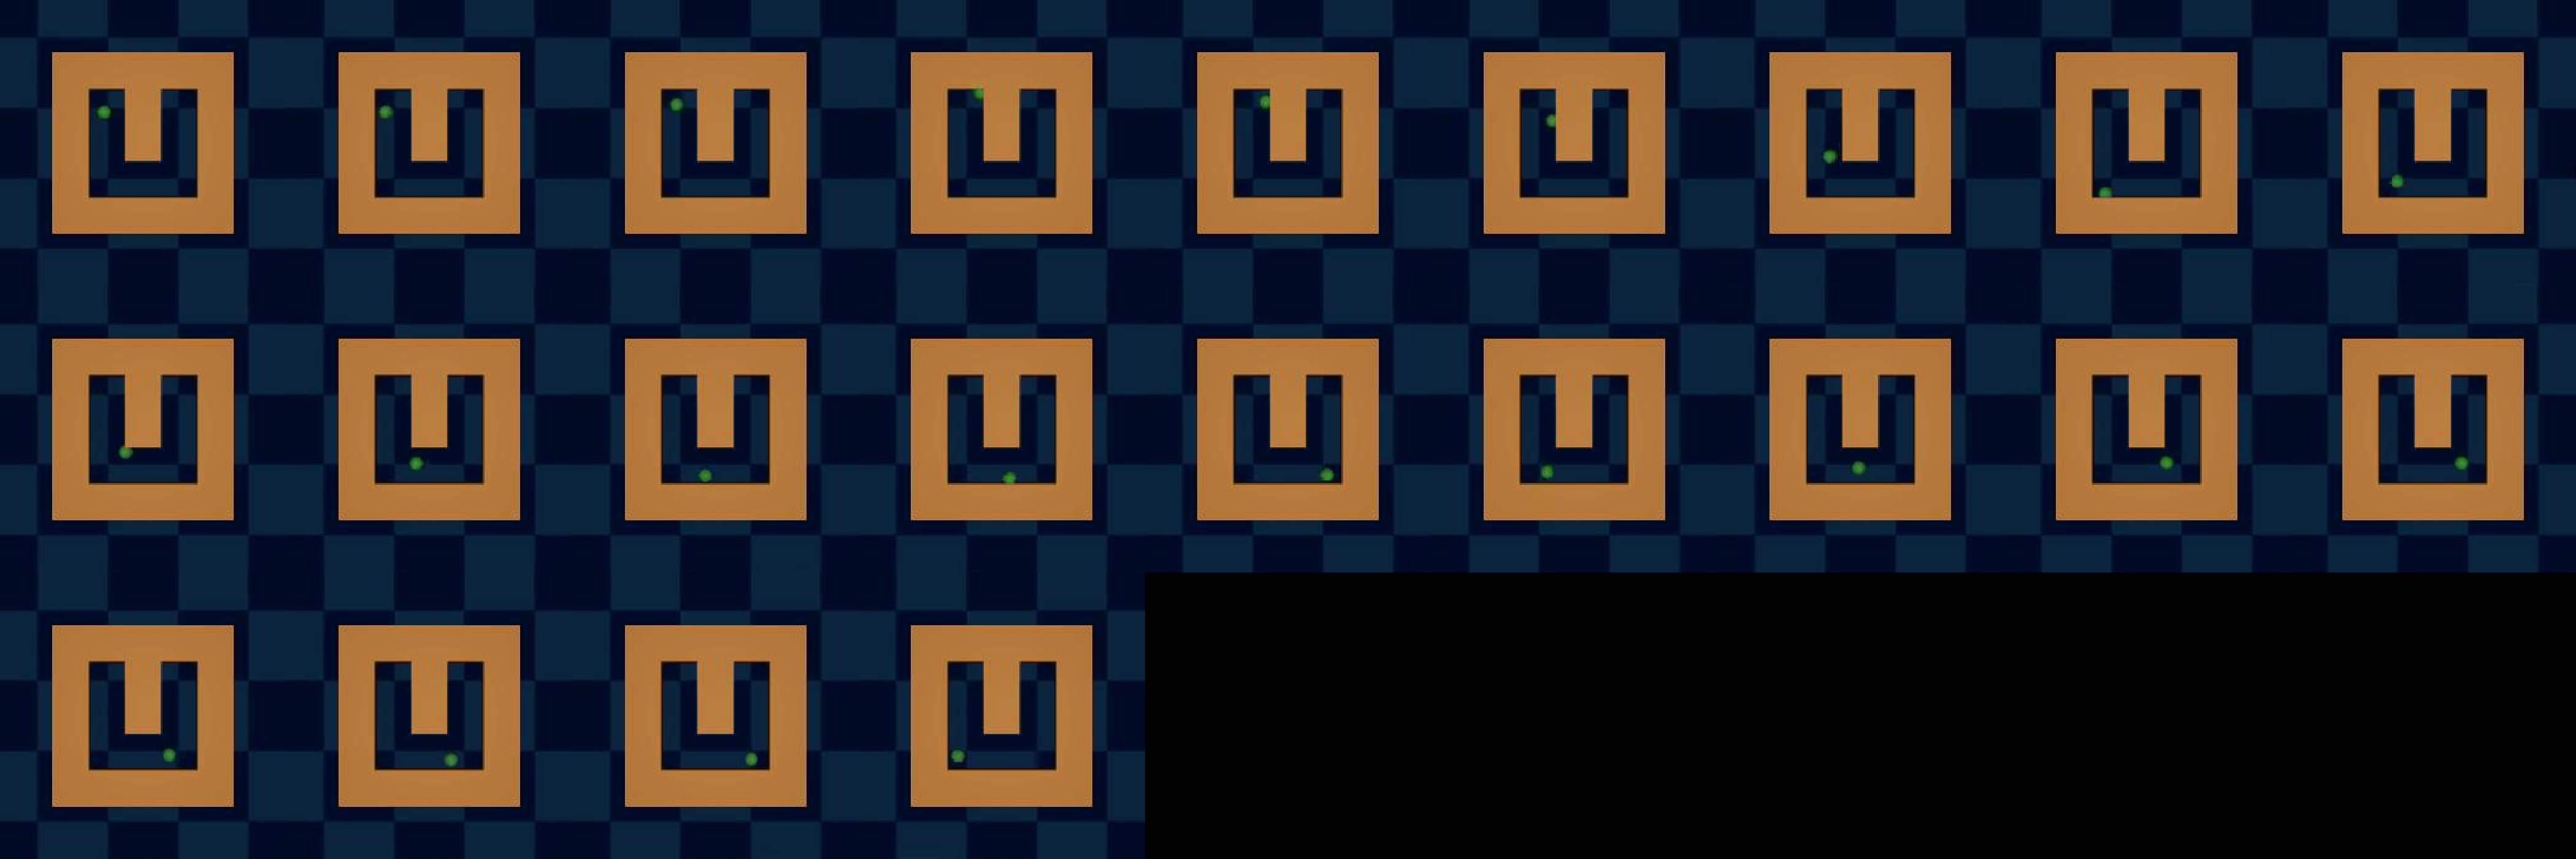
\includegraphics[width=\textwidth]{images/plan20_0_success_grid.pdf}
        \caption{With straightening, the agent reaches the target within given step limit.}
    \end{subfigure}
    \begin{subfigure}[t]{\textwidth}
        \centering
        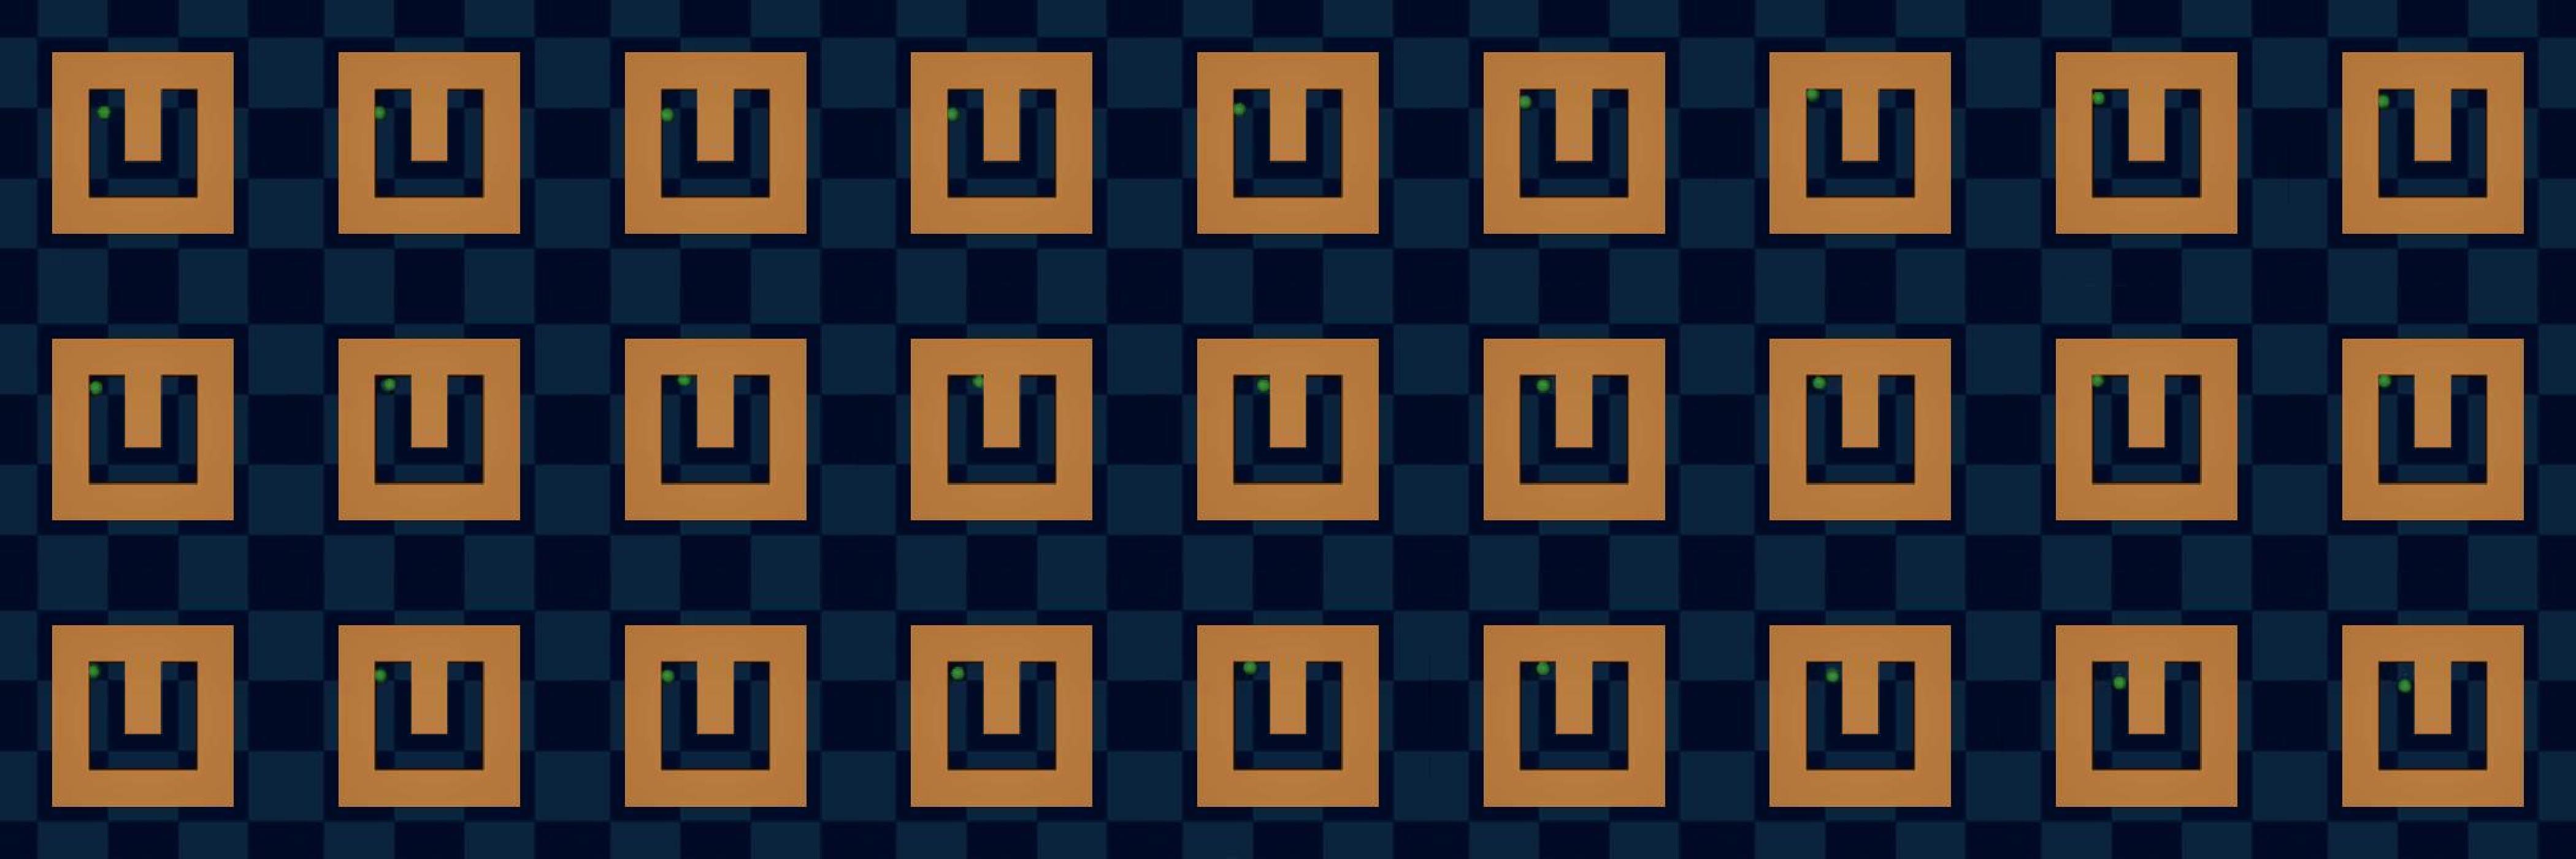
\includegraphics[width=\textwidth]{images/plan25_0_failure_grid.pdf}
        \caption{Without straightening, the agent gets stuck at the corner.}
    \end{subfigure}
\caption{Comparison of Planning Trajectories in Teleported-PointMaze. The frames were masked by black after reaching the target.
}
\label{img:teleport_str_comp}
\end{figure*}


